\documentclass[11pt]{article}
%% Packages:

\usepackage{amsmath}
\usepackage[document]{ragged2e}
\usepackage{titlesec}
\usepackage{float}
\usepackage{graphicx}
\usepackage{caption}
\usepackage{subcaption}
\usepackage[dvipsnames]{xcolor}
\usepackage[T1]{fontenc}
\usepackage{helvet}
\usepackage[hidelinks]{hyperref}
\usepackage[margin=2cm]{geometry}
\usepackage{amssymb}
\usepackage{enumitem}
\usepackage{comment}
\usepackage{soul}

%% Personalized adjustements: 

% Math operator:
\DeclareMathOperator{\sech}{sech}

% VUB colors: 
\definecolor{orange}{RGB}{234, 82, 0} 
\definecolor{blue}{RGB}{26, 55, 101}

% Margins:
\addtolength{\skip\footins}{0.3 cm}
\renewcommand*\footnoterule{}

% Adjustement of section, subsection & subsubsection: 

\titleformat{\section}[block]
{\normalfont\Large\bfseries \fontfamily{phv}\selectfont \color{orange}}
{\thesection}{0.5cm}{}

\titleformat{\subsection}[block]
{\normalfont\large\bfseries \fontfamily{phv}\selectfont \color{blue}}
{\thesubsection}{0.5cm}{}

\titleformat{\subsubsection}[block]
{\normalfont\small\bfseries \fontfamily{phv}\selectfont \color{blue}}
{\thesubsubsection}{0.5cm}{}
\usepackage{setspace}
\usepackage{graphicx}
\usepackage{subcaption}
\usepackage{parskip}
\usepackage{indentfirst}
\graphicspath{{Images/}}
%\setlength{\parindent}{1.5em}
\usepackage{float}
\onehalfspacing

\begin{document}
	\justifying
	
	\begin{titlepage}
	\begin{center}
            \begin{figure}
                \centering
                
\includegraphics[scale=0.3]{Images/logo.png}
            \end{figure}
		\vspace*{\fill}
            \normalsize
            {\fontfamily{phv}\selectfont
            \textcolor{blue}{\textbf{ELEC-H401}}}\\
            \vspace{0.2cm}
		\Huge
            {\fontfamily{phv}\selectfont
            \textcolor{orange}{Design and Simulation of a DVB-C Transmission Chain}}\\
        \end{center}
	\begin{center}	
		\vspace{0.5cm}
            \Large
            {\fontfamily{phv}\selectfont
			\textcolor{blue}{\textbf{Hadislam Satouev\\
                                 	 Cédric Sipakam
             }}}\\
	\end{center}
        \vspace*{\fill}
        \begin{FlushRight}
            {\fontfamily{phv}\selectfont
            \textcolor{orange}{Professor}}\\
            {\fontfamily{phv}\selectfont
            \textcolor{blue}{François Horlin}}\\
            \vspace{0.6cm}
            {\fontfamily{phv}\selectfont
            \textcolor{orange}{Teaching Assistants}}\\
            {\fontfamily{phv}\selectfont
            \textcolor{blue}{
                ....\\
                 ....
            }}\\
            \vspace{0.6cm}
            {\fontfamily{phv}\selectfont
            \textcolor{orange}{Academic Year}}\\
            {\fontfamily{phv}\selectfont
            \textcolor{blue}{2024 - 2025}}\\
            \vspace{0.6cm}
            {\fontfamily{phv}\selectfont
            \textcolor{orange}{Faculty}}\\
            {\fontfamily{phv}\selectfont
            \textcolor{blue}{Electrical Engineering}}
        \end{FlushRight}



\end{titlepage}
	\tableofcontents
	\newpage
	\listoffigures
	
	\newpage
	\section*{Introduction}{\addcontentsline{toc}{section}{Introduction}}
	This project focuses on designing and simulating a Digital Video Broadcasting Cable transmission chain using Matlab.
	The main goal is to model and analyze the components of a typical modem. The first part of this project includes establishing an optimal communication chain over an ideal Additive White Gaussian Noise channel, mapping the signal into symbols, Nyquist filtering, and evaluating the performance of the system through Bit Error Rate simulations for Quadrature Amplitude Modulation signals. The second part revolves around the design and assessment of time and frequency synchronization algorithms. This encompasses evaluating the impact of synchronization errors such as carrier phase and frequency offset and sample time shift. The algorithms used for this purpose are the Gardner Algorithm for time recovery, and a differential cross-correlator for joint frame and frequency acquisition. Afterwards, their effectiveness is demonstrated \textcolor{red}{through convergence analysis and residual error evaluation (double check)}. \textcolor{red}{The study also explores phase interpolation techniques to mitigate remaining phase drifts. Finally, the project aims to validate the simulated chain through real-life experimentation on a Hybrid Fiber-Coax setup using Adalm-Pluto hardware, and to compare the simulated performance with experimental observations.}
	
	
	\section{Optimal Communication Chain over the Ideal Channel}
	\subsection{Communication Chain}
	\begin{figure}[H]
		\centering
		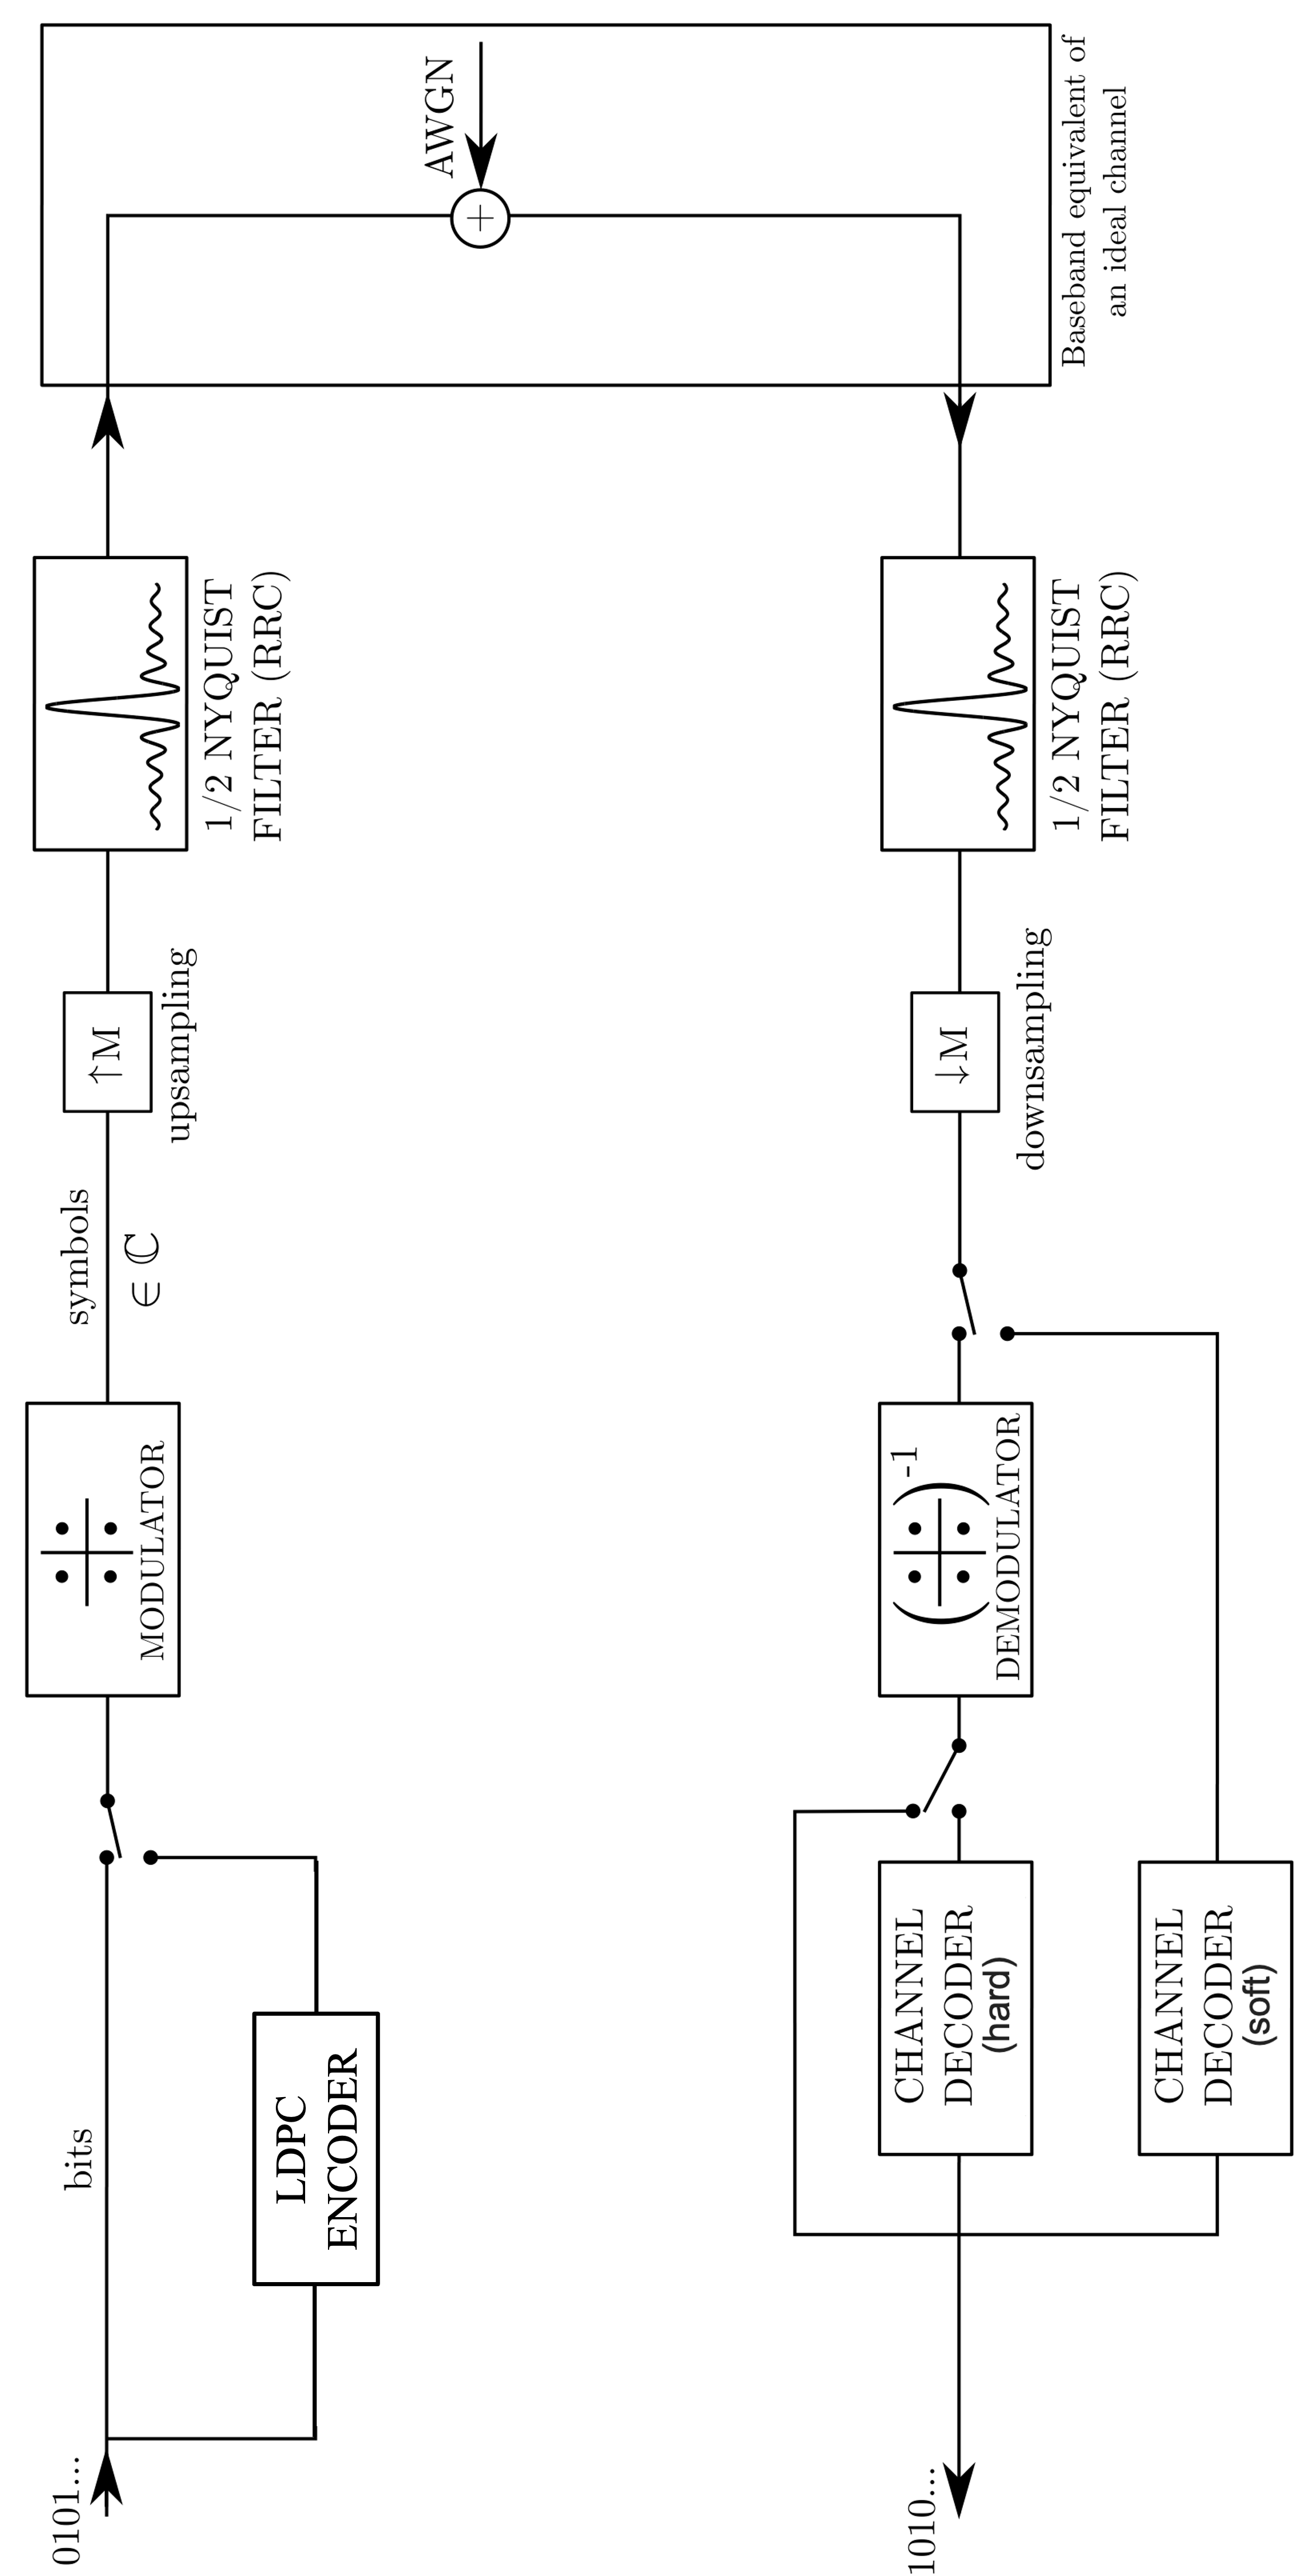
\includegraphics[angle=-90, width=0.7\linewidth]{Images/com-chain}
		\caption{Block diagram of the communication system.}
		\label{fig:com-chain}
	\end{figure}
	Figure \ref{fig:com-chain} shows the simulated DVB-C baseband communication chain. A transmitter generates a bit-stream, maps it to QAM symbols, up-samples, and shapes them with a half-root Nyquist filter to limit bandwidth. The receiver employs a matched half-root Nyquist filter to maximize SNR, then down-samples at symbol instances, and demapps samples to estimate the transmitted bit-stream.
	\par
	In this project, the Low Density Parity Check Encoder is not implemented, and the algorithms for symbol mapping and demapping were provided.
	
	\subsection{Bit Generation and Symbol Mapping and Demapping}
	Mapping bit-streams to complex symbols enhances spectral efficiency (more bits/symbol per bandwidth). Symbol demapping in the receiver estimates the bit sequence from noisy symbols using the Maximum Likelihood (ML) criterion. ML selects the constellation symbol $\underline{s}_{m}$ minimizing Euclidean distance to the received sample $\underline{r}$:
	\begin{equation}
		\tilde{\underline{s}}_{m}^{ML} = \arg\min_{\underline{s}_{m}} \left(\sum_{k=1}^{K}(r_{k}-s_{mk})^{2}\right)
	\end{equation}
	Where:
	\begin{itemize}
		\item $\tilde{\underline{s}}_{m}^{ML}$ is the estimated symbol using the ML criterion.
		\item $\underline{r} = [r_1, r_2, \dots, r_K]^T$ is the received vector after demodulation.
		\item $\underline{s}_{m} = [s_{m1}, s_{m2}, \dots, s_{mK}]^T$ is the vector representing the $m$-th possible transmitted symbol.
	\end{itemize}
	Minimizing squared Euclidean distance is equivalent to maximizing $\ln p(\underline{r}|\underline{s}_{m})$ for an Additive White Gaussian Noise (AWGN) channel, where $p(\underline{r}|\underline{s}_{m})$ is the conditional probability of receiving vector $\underline{r}$ given symbol $\underline{s}_m$ was sent.
	
	\subsection{Nyquist Filtering}
	Mapped complex symbols $I[k]$ are up-sampled by OSF $> 1$ and passed through a pulse shaping filter $g(t)$ to:
	\begin{enumerate}
		\item Limit transmitted signal bandwidth.
		\item Control inter-symbol interference.
	\end{enumerate}
	
	\subsubsection{Half-Root Nyquist Filter Design and Matched Filtering}
	For optimal ISI cancellation and SNR maximization, a root-raised cosine (RRC) filter $g(t)$ is used for pulse shaping. The receiver uses a matched filter $g^*(-t)$. Their convolution, $h(t) = g(t) \otimes g^*(-t)$, is the overall channel response, designed to satisfy the Nyquist zero ISI criterion at sampling intervals $T_{symb}$ (normalized $h(t)$):
	\begin{equation}
		h(kT_{symb}) = \begin{cases}
			1 & k=0 \\
			0 & k \neq 0
		\end{cases}
		\label{eq:nyquist_criterion_part1}
	\end{equation}
	\par
	The RRC filter $g(t)$ is derived from a raised-cosine (RC) filter with transfer function $H(f)$. The RRC frequency response is $G(f) = \sqrt{H(f)}$, and $g(t) = \mathcal{F}^{-1}\{G(f)\}$. $H(f)$ is given by:
	\begin{equation}
		H(f) = \begin{cases}
			T_{symb} & 0 \le |f| < \frac{1-\beta}{2T_{symb}} \\      
			\frac{T_{symb}}{2} \left(1 + \cos\left[\frac{\pi T_{symb}}{\beta}\left(|f| - \frac{1-\beta}{2T_{symb}}\right)\right]\right) & \frac{1-\beta}{2T_{symb}} \le |f| \le \frac{1+\beta}{2T_{symb}} \\      
			0 & |f| > \frac{1+\beta}{2T_{symb}}
		\end{cases}
		\label{eq:rc_response_part1}
	\end{equation}
	
	\subsubsection{Filter Properties and Inter-Symbol Interference Cancellation}
	\begin{figure}[H]
		\centering
		\begin{subfigure}[b]{0.48\textwidth}
			\centering
			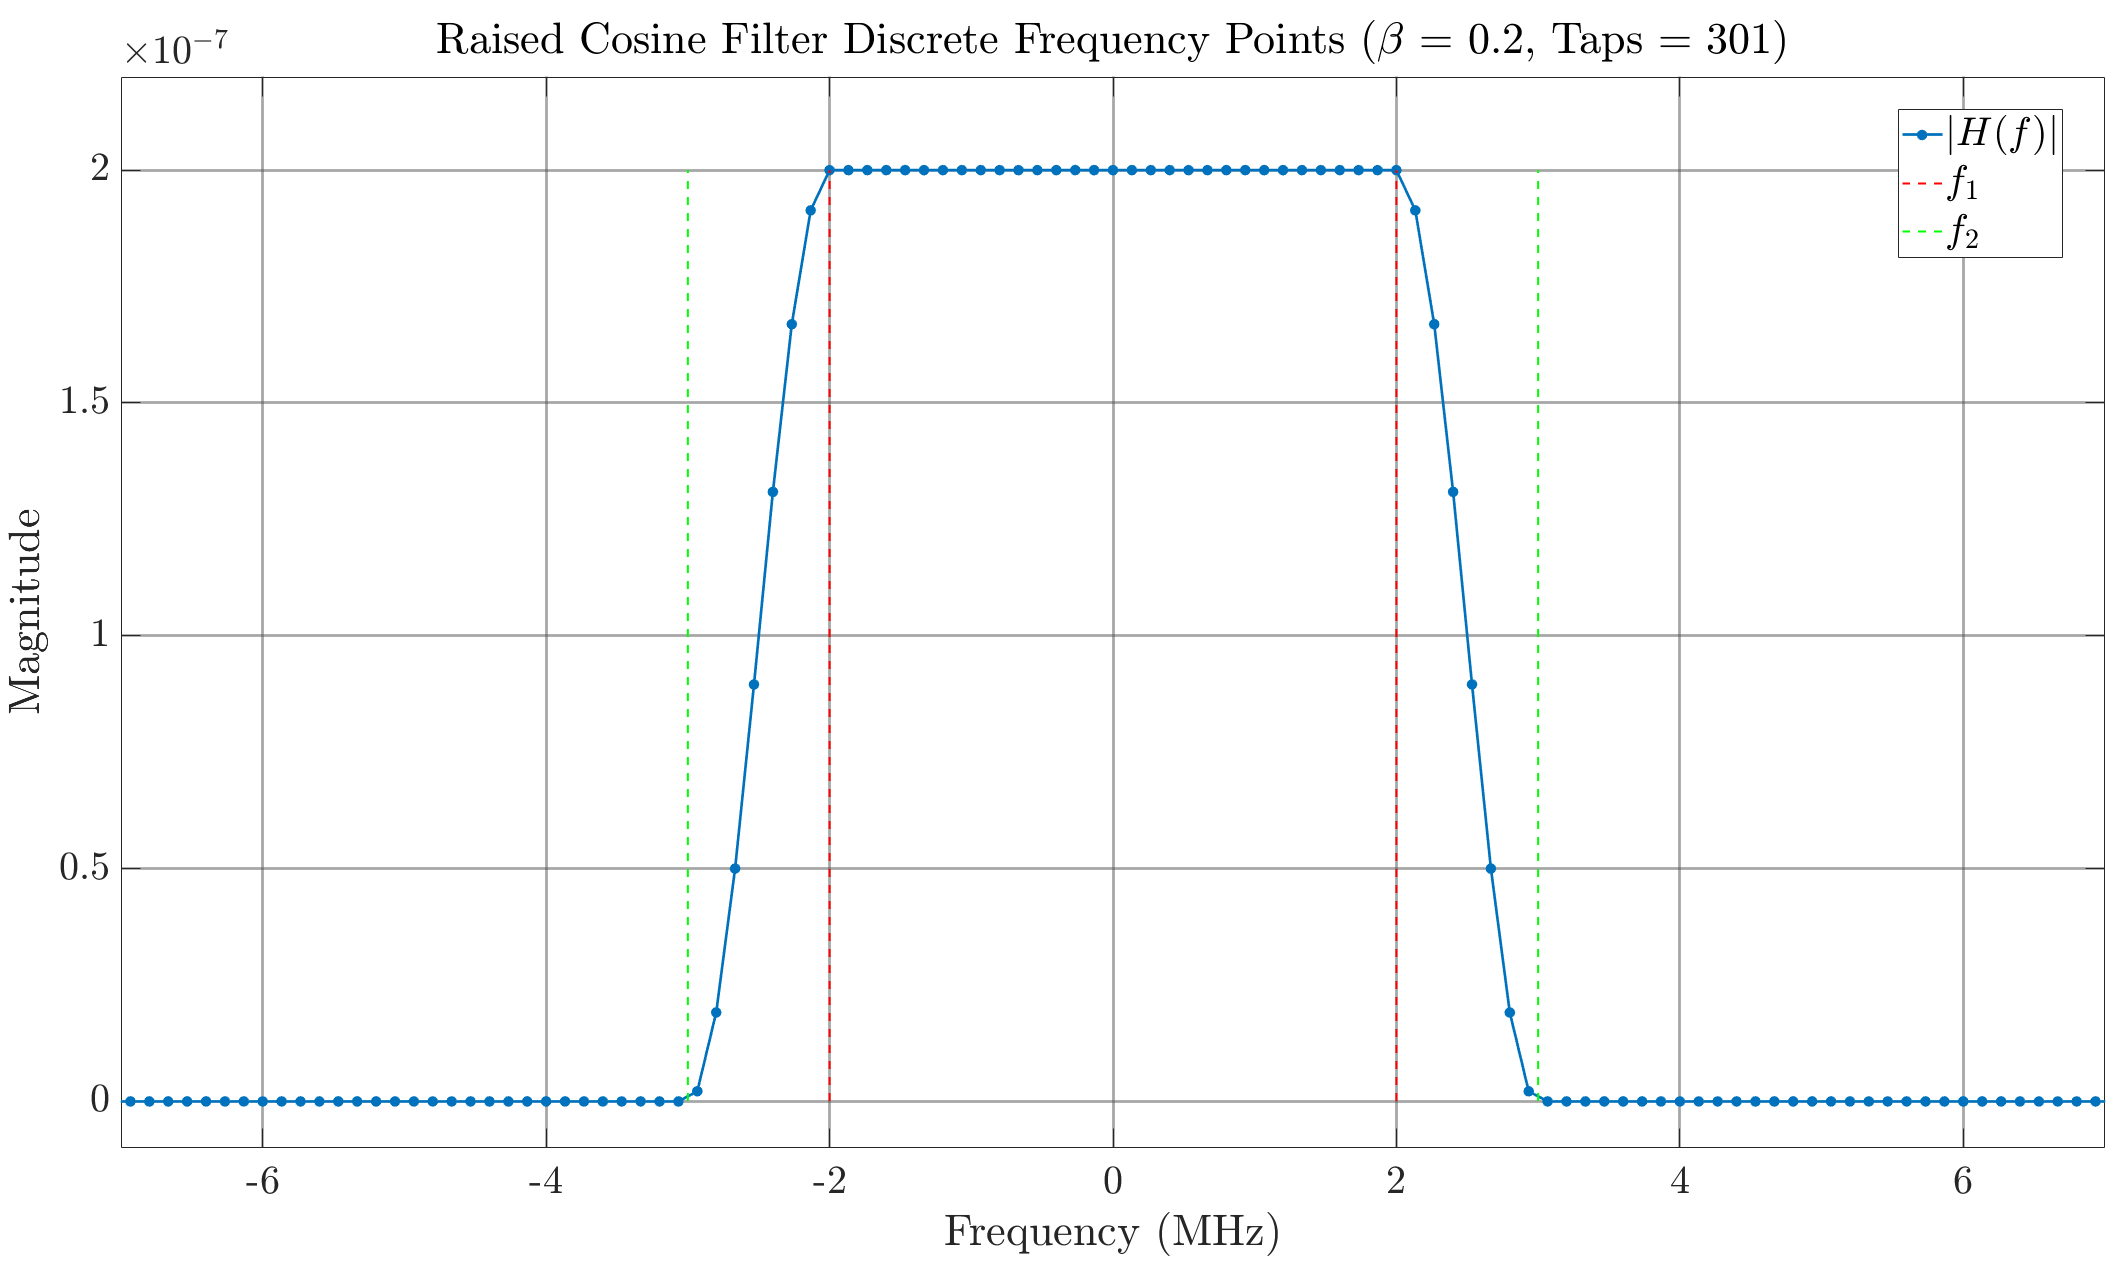
\includegraphics[width=\linewidth]{Images/h-rc-freq}
			\caption{Simulated Raised Cosine Filter Frequency Response from ($\beta = 0.2$, $taps = 301$, $OSF = 8$).}
			\label{fig:h-rc-freq}
		\end{subfigure}
		\hfill % This will add horizontal space between the subfigures
		\begin{subfigure}[b]{0.48\textwidth}
			\centering
			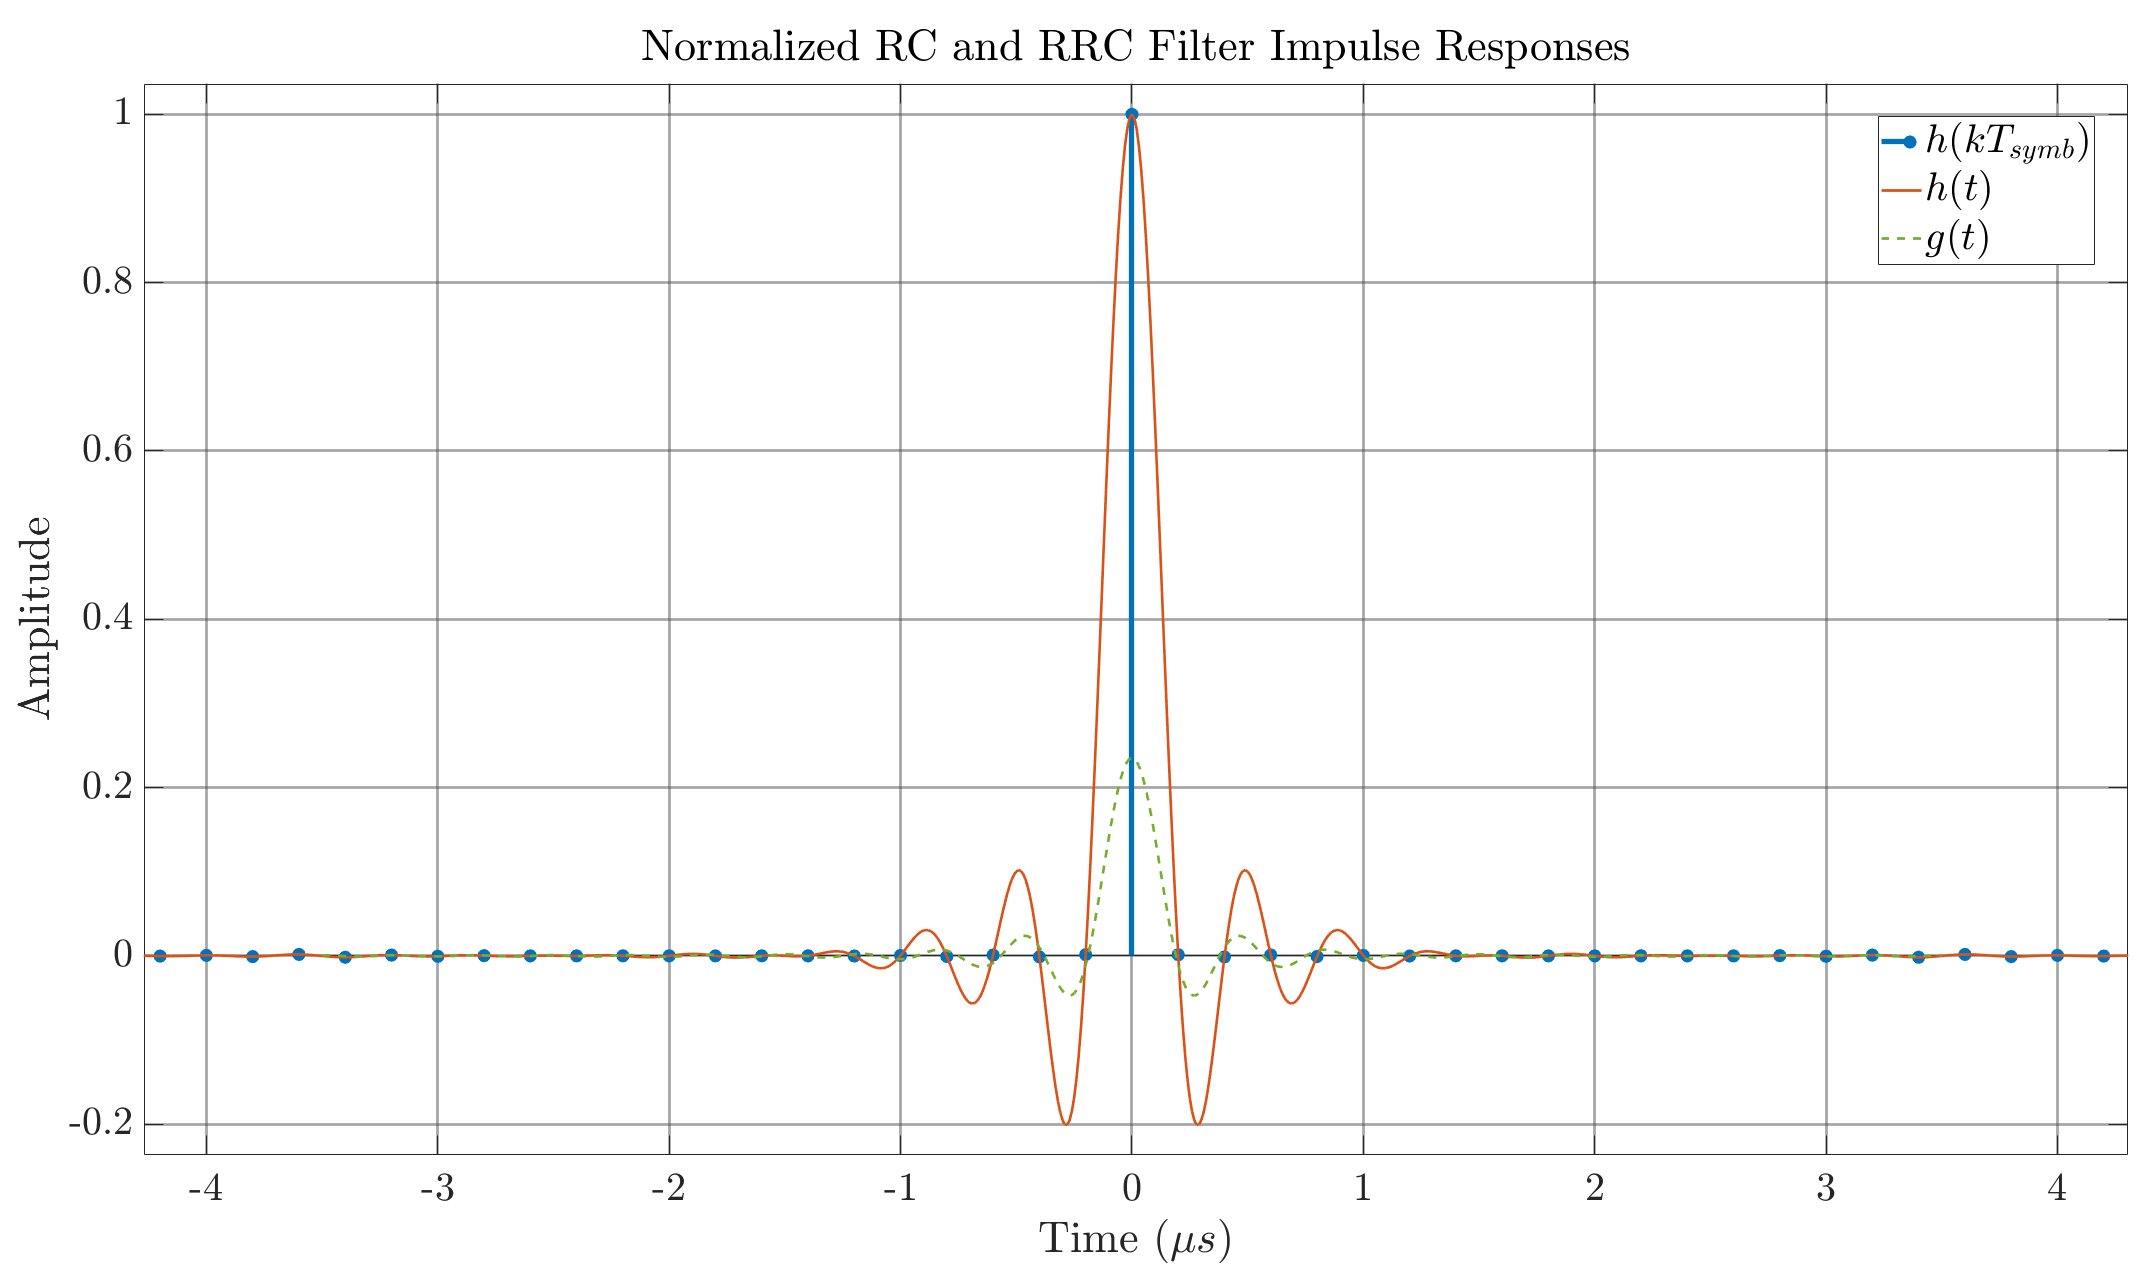
\includegraphics[width=\linewidth]{Images/h-rc}
			\caption{Simulated Normalized RC and RRC filter Impulse Responses, with $h(kT_{symb})$ illustrating ISI cancellation.}
			\label{fig:h-rc}
		\end{subfigure}
		\caption{Simulated characteristics of the Nyquist filtering: frequency response (left) and impulse responses (right).}
		\label{fig:nyquist-filter-combined}
	\end{figure}
	
	The overall RC filter $h(t)$ confines signal energy to a communication bandwidth of $R_{symb}(1+\beta)$. For project parameters ($R_{symb} = 5 \text{ Msymb/s}$ and $\beta = 0.2$), this bandwidth is $6 \text{ MHz}$. Figure \ref{fig:h-rc-freq} shows the simulated $H(f)$, confirming spectral confinement with its passband, roll-off, and stopband.
	
	In the time domain, $h(t)$ when sampled at $T_{symb}$ intervals approximates a Dirac delta, satisfying Eq. \ref{eq:nyquist_criterion_part1} for zero ISI. Figure \ref{fig:h-rc} shows the simulated $h(t)$; stems at $h(kT_{symb})$ (unity at $t=0$, zero elsewhere) confirm ISI elimination by nullifying other symbols' contributions at the optimal sampling instant.
	
	
	\subsection{Noise Addition and Performance Evaluation}
	AWGN, representing cumulative interference and thermal noise, limits performance. In the simulated baseband model, the received signal $r(t)$ is $s(t)$ (output of $g(t)$) plus complex baseband noise $n(t)$:
	\begin{equation}
		r(t) = s(t) + n(t)
	\end{equation}
	\par
	The noise $n(t)$ is complex Gaussian, with independent real/imaginary components, each with Power Spectral Density (PSD) $N_0/2$. After matched filtering with $g^*(-t)$ and sampling at $t = kT_{symb}$, the $k$-th received sample is $y[k] = (r(t) \otimes g^*(-t))|_{t=kT_{symb}}$. Since the signal component of $r(t)$ is $\sum_m I[m]g(t-mT_{symb})$, and $h(t) = g(t) \otimes g^*(-t)$ satisfies the Nyquist criterion (Eq. \ref{eq:nyquist_criterion_part1}, with $h(0)$ normalized to 1):
	\begin{align}
		y[k] &= \left( \left(\sum_m I[m]g(t-mT_{symb})\right) \otimes g^*(-t) \right)\Big|_{t=kT_{symb}} + (n(t) \otimes g^*(-t))|_{t=kT_{symb}} \nonumber \\
		&= \sum_m I[m]h((k-m)T_{symb}) + n_o[k] \nonumber \\
		&= I[k]h(0) + \sum_{m \neq k} I[m]h((k-m)T_{symb}) + n_o[k] \nonumber \\
		&= I[k] + n_o[k] \label{eq:yk_plus_noise}
	\end{align}
	where $I[k]$ is the transmitted complex symbol and $n_o[k] = (n(t) \otimes g^*(-t))|_{t=kT_{symb}}$ is the filtered and sampled noise. The noise samples $n_o[k]$ are complex Gaussian, as $n(t)$ is white Gaussian and matched filtering is linear. Real/imaginary components of $n_o[k]$ are independent, each with variance $\sigma^2 = N_0/2$.
	
	System performance is evaluated by simulating Bit Error Rate (BER) vs. $E_b/N_0$, based on Eq. \ref{eq:yk_plus_noise}. To simulate at a specific $E_b/N_0$, noise power $n_o[k]$ is set relative to signal power. Average symbol energy $E_s = \text{E}\left[|I[k]|^2\right]$. Average bit energy $E_b = E_s / b = E_s / \log_2 M$ (M-QAM, $b$ bits/symbol). Then, $N_0 = E_b / (E_b/N_0)_{\text{target}}$. The complex noise $n_o[k]$ added per Eq. \ref{eq:yk_plus_noise} has total variance $N_0$ (real/imaginary components each $N_0/2$).
	
	Experimental BER is:
	\begin{equation}
		\text{BER}_{\text{exp}} = \frac{\text{Number of erroneously detected bits}}{\text{Total number of transmitted bits}}
	\end{equation}
	Simulated BER vs. $E_b/N_0$ is compared to theoretical $P_b$ for M-QAM (square, Gray coded, moderate/high $E_b/N_0$):
	\begin{equation}
		P_b \approx \frac{4}{\log_2 M} \left(1 - \frac{1}{\sqrt{M}}\right) Q\left(\sqrt{\frac{3 (\log_2 M)}{M-1} \frac{E_s}{N_0}}\right) = \frac{4}{\log_2 M} \left(1 - \frac{1}{\sqrt{M}}\right) Q\left(\sqrt{\frac{3 (\log_2 M)^2}{M-1} \frac{E_b}{N_0}}\right)
		\label{eq:Pb_MQAM_Eb_cont_final}
	\end{equation}
	where $Q(x) = \frac{1}{\sqrt{2\pi}} \int_x^\infty e^{-u^2/2} du$.
	
	Figure \ref{fig:ber-mod_cont} shows simulated BER for various QAMs, illustrating the spectral vs. power efficiency trade-off: higher-order modulations offer higher data rates but need more power for the same BER.
	
	\begin{figure}[H]
		\centering
		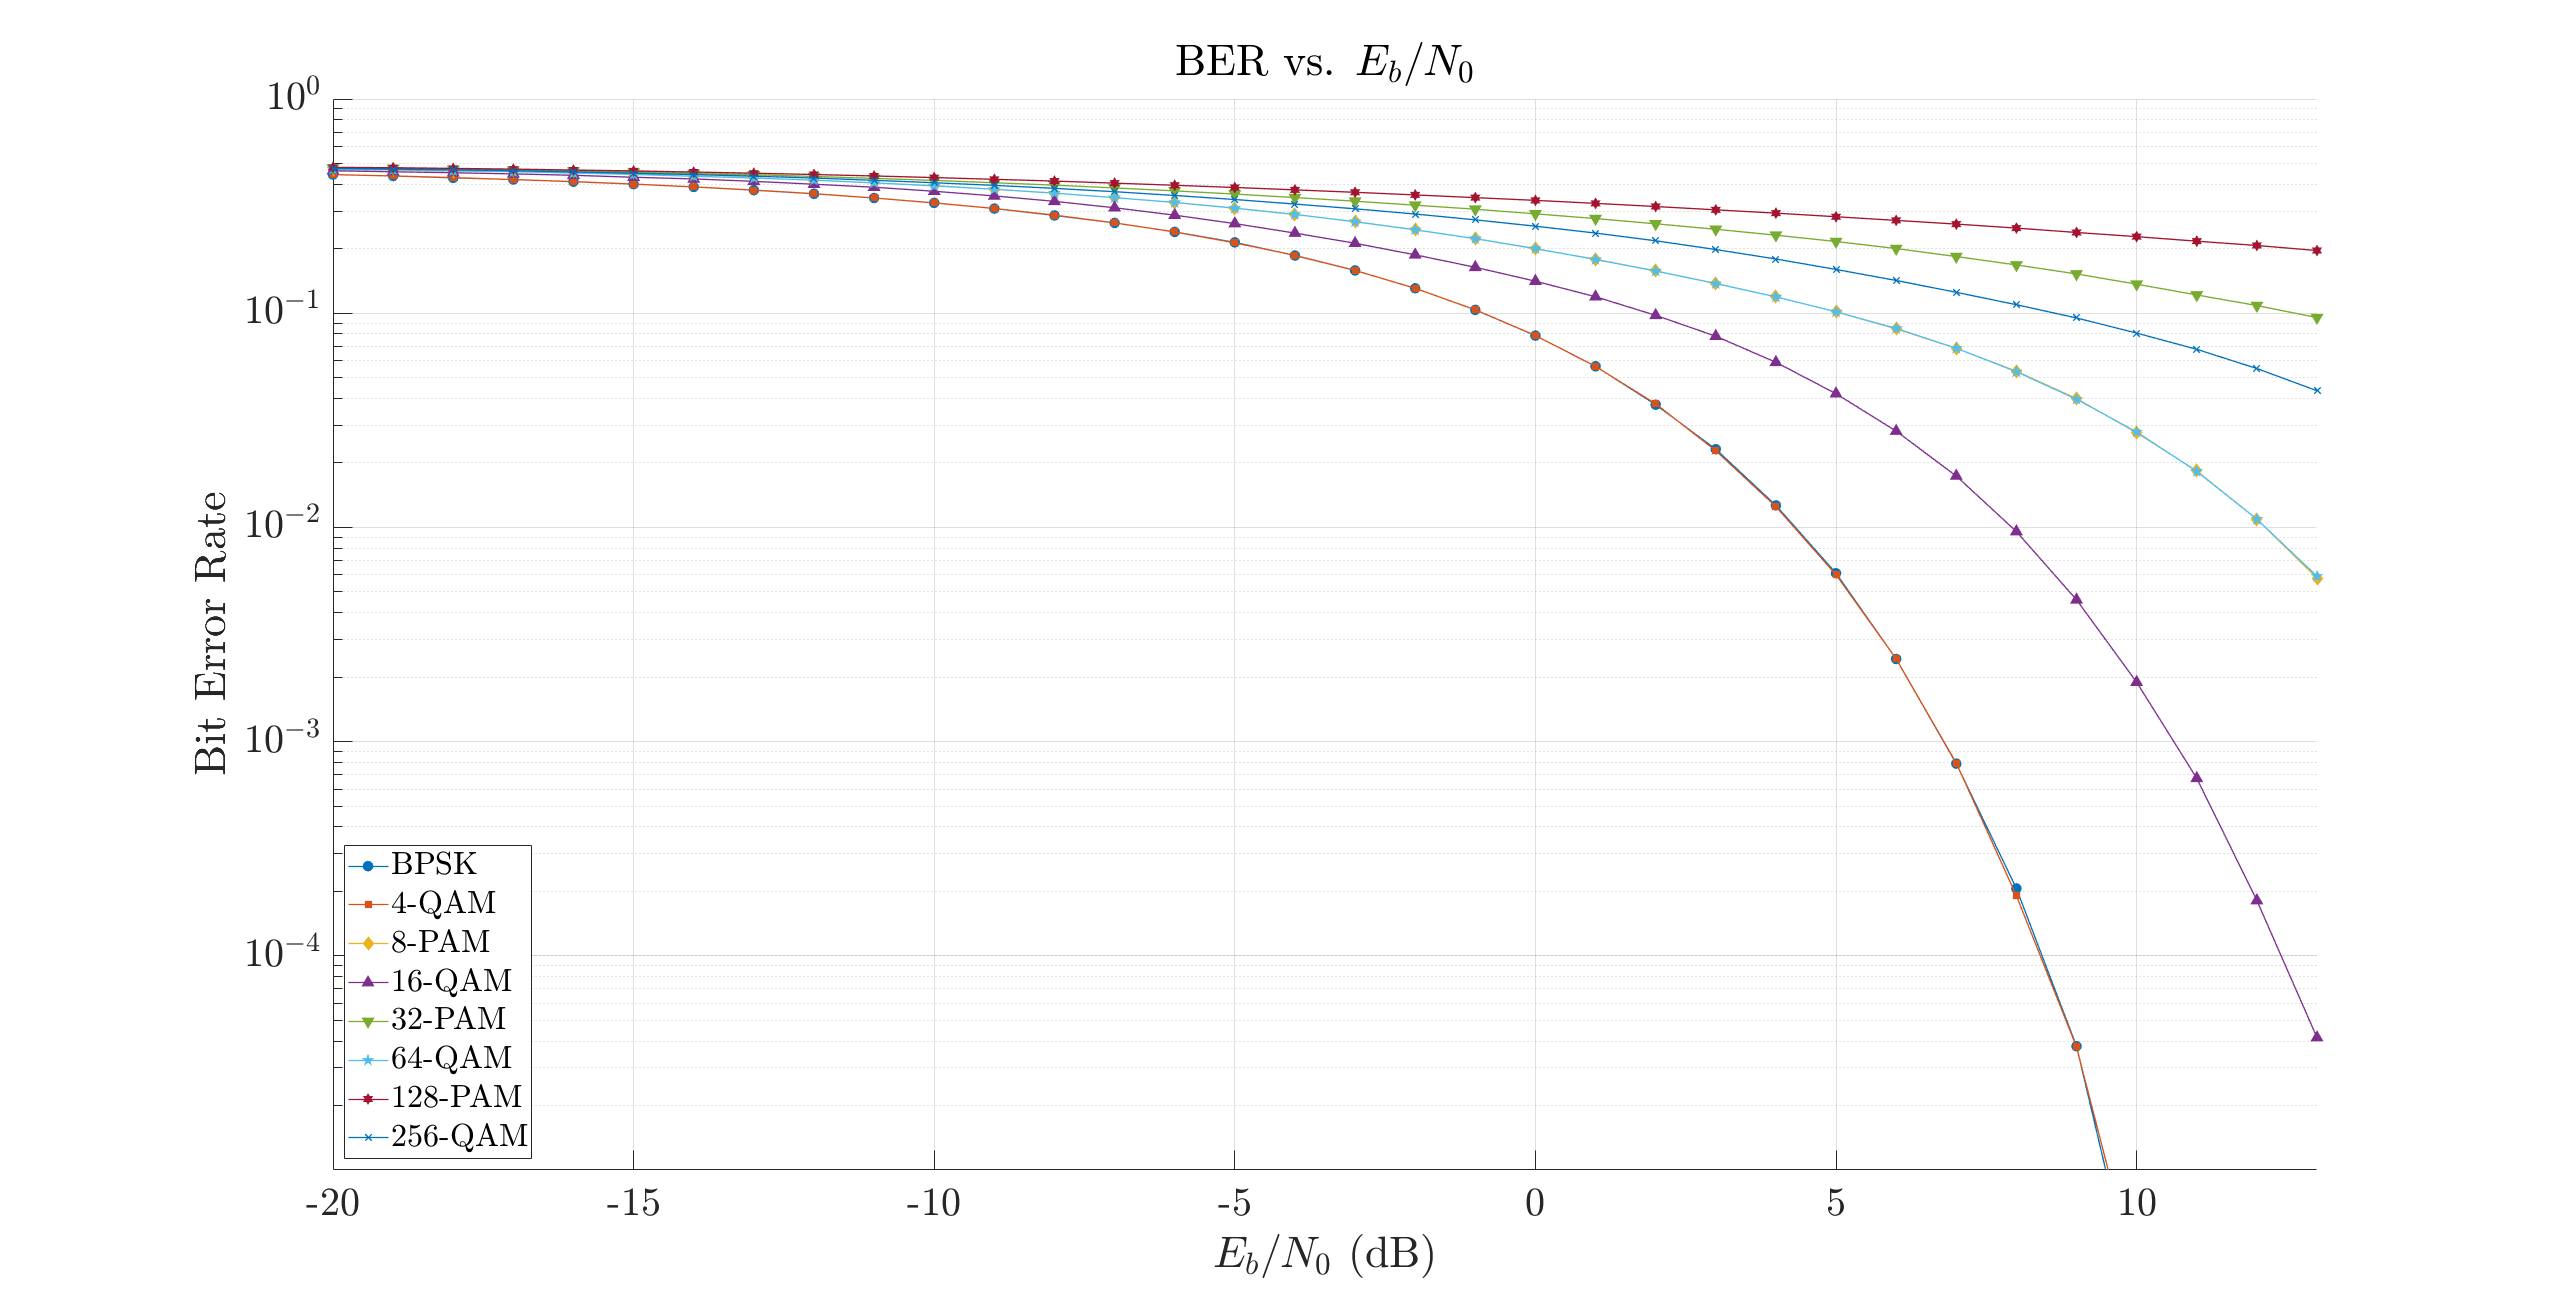
\includegraphics[width=0.8\linewidth]{Images/ber-mod.png}
		\caption{Simulated BER vs. $E_b/N_0$ for various modulation types}
		\label{fig:ber-mod_cont}
	\end{figure}
	
	Figure \ref{fig:constellations-noise_cont} shows AWGN's effect on 16-QAM constellations. Figure \ref{fig:const-noisy_cont} displays symbols $s(t)+n(t)$ pre-matched filter. Post-matched filtering and downsampling ($y[k]=I[k]+n_o[k]$), symbols in Fig. \ref{fig:const-filtered-down_cont} cluster around ideal points, validating the matched filter's SNR maximization.
	
	\begin{figure}[H]
		\centering
		\begin{subfigure}{0.48\textwidth}
			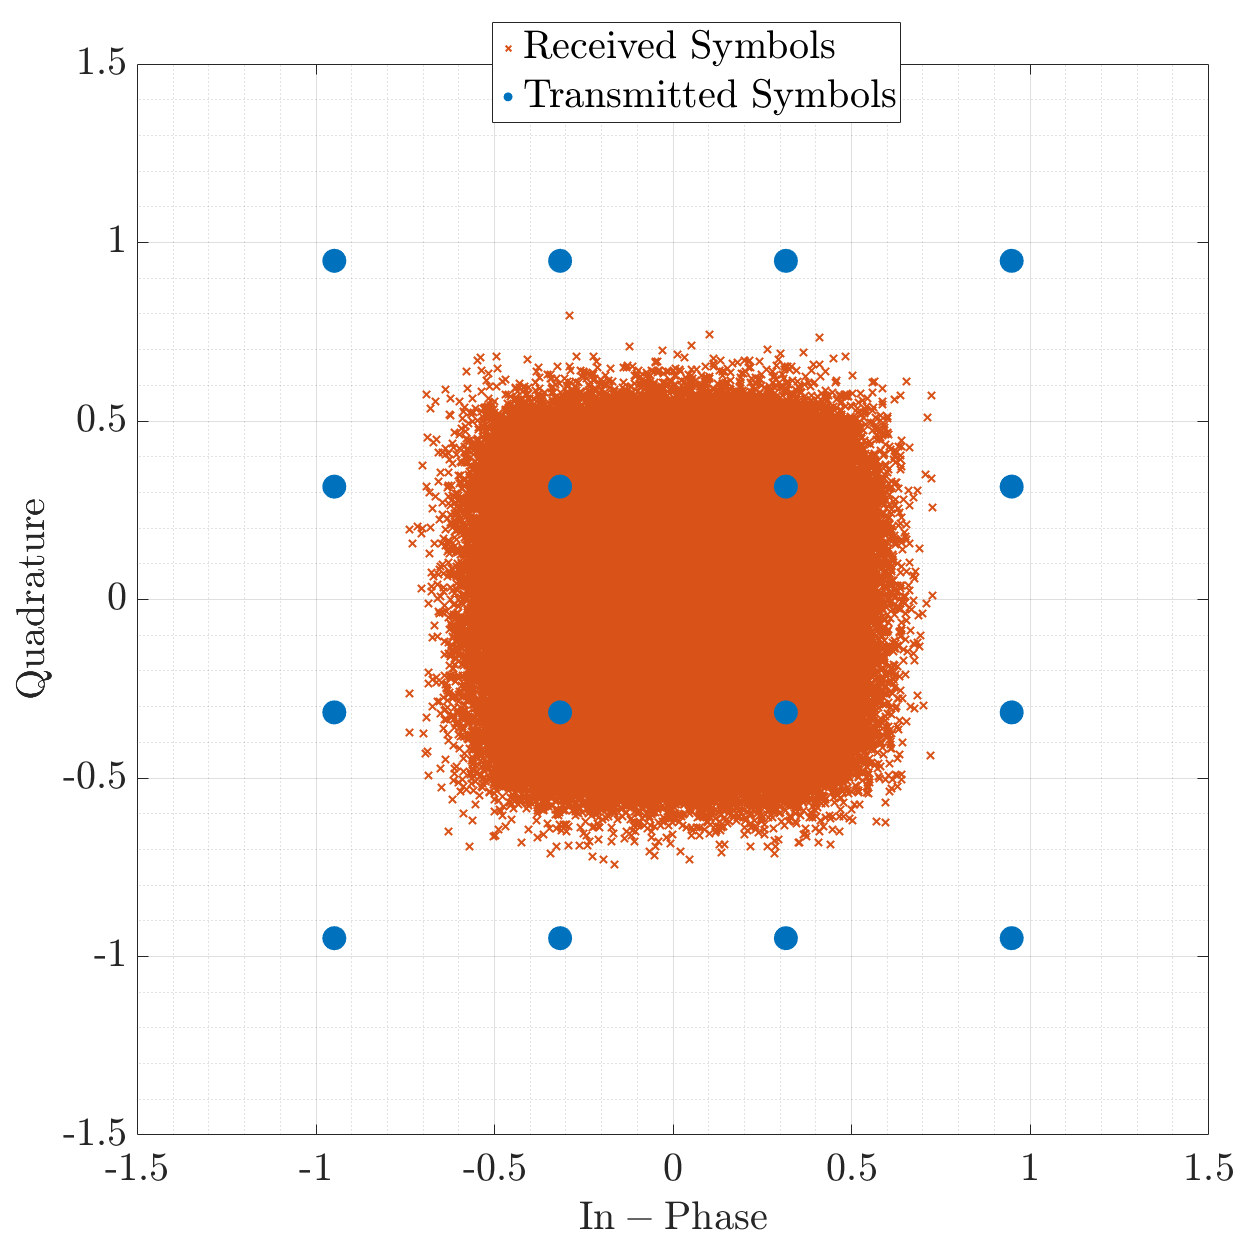
\includegraphics[width=\linewidth]{Images/const-noisy.png}
			\caption{Simulated noisy 16-QAM symbols before matched filter.}
			\label{fig:const-noisy_cont}
		\end{subfigure}\hfill
		\begin{subfigure}{0.48\textwidth}
			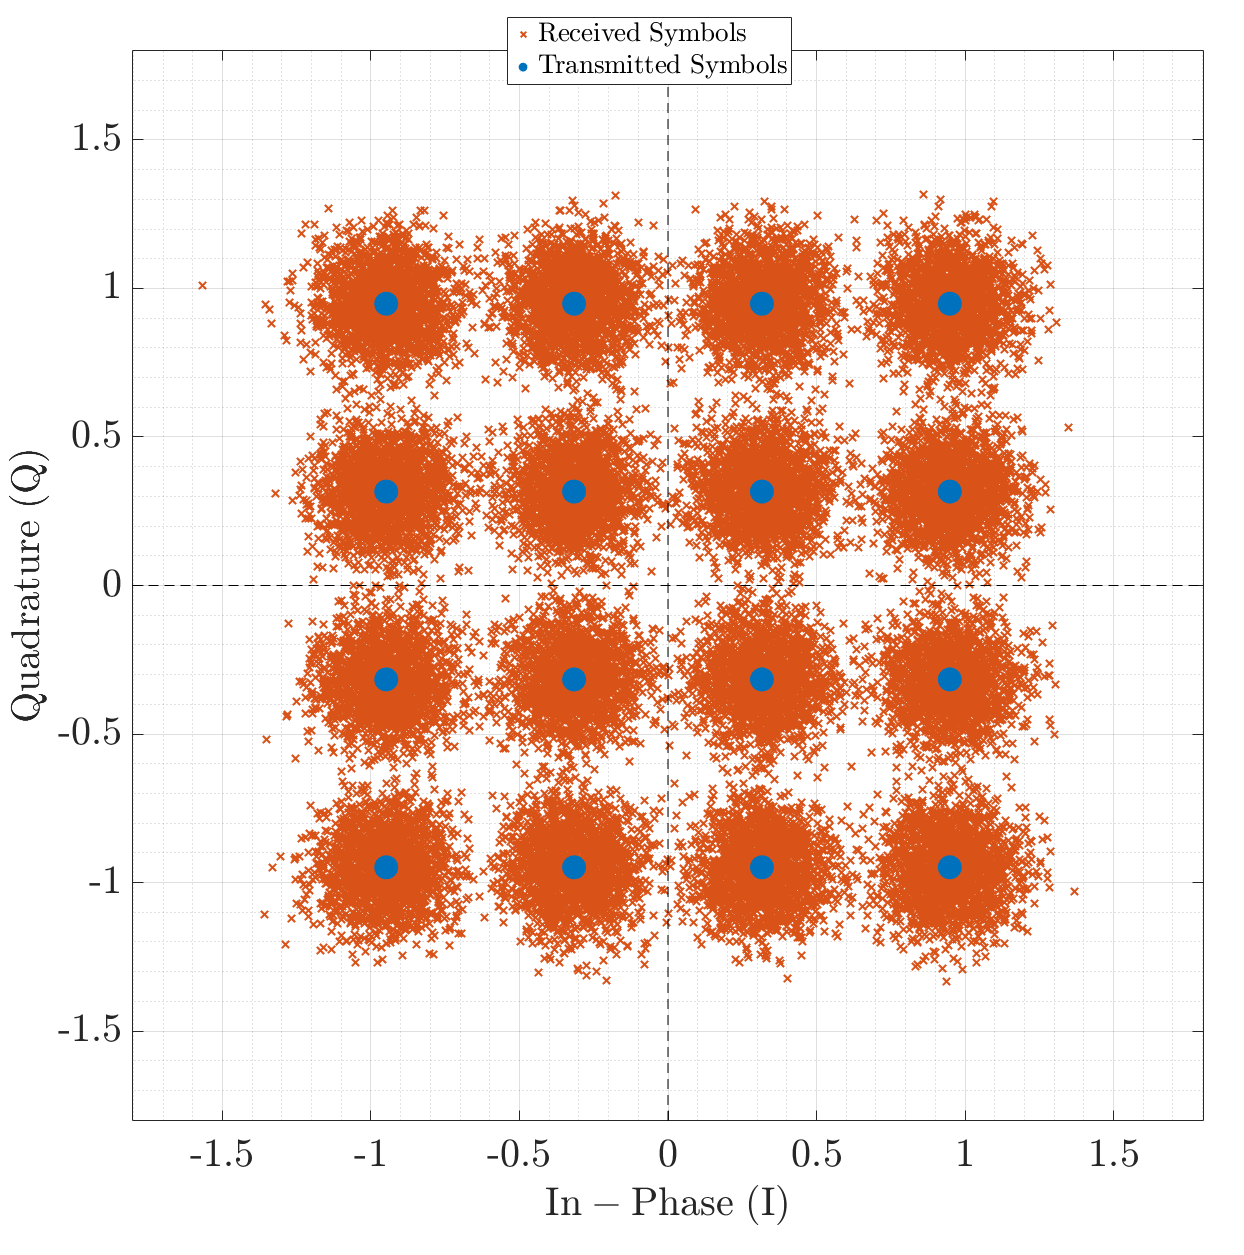
\includegraphics[width=\linewidth]{Images/const-filtered-down.png}      
			\caption{Simulated 16-QAM symbols after matched filtering and downsampling.}
			\label{fig:const-filtered-down_cont}
		\end{subfigure}
		\caption{Simulation - Effect of AWGN and matched filtering on a 16-QAM constellation ($\frac{E_b}{N_0} = 15$ dB)}
		\label{fig:constellations-noise_cont}
	\end{figure}
	
	\section{Time and Frequency Synchronization}
	\subsection{The Problem of Synchronization}
	\begin{figure}[H]
		\centering
		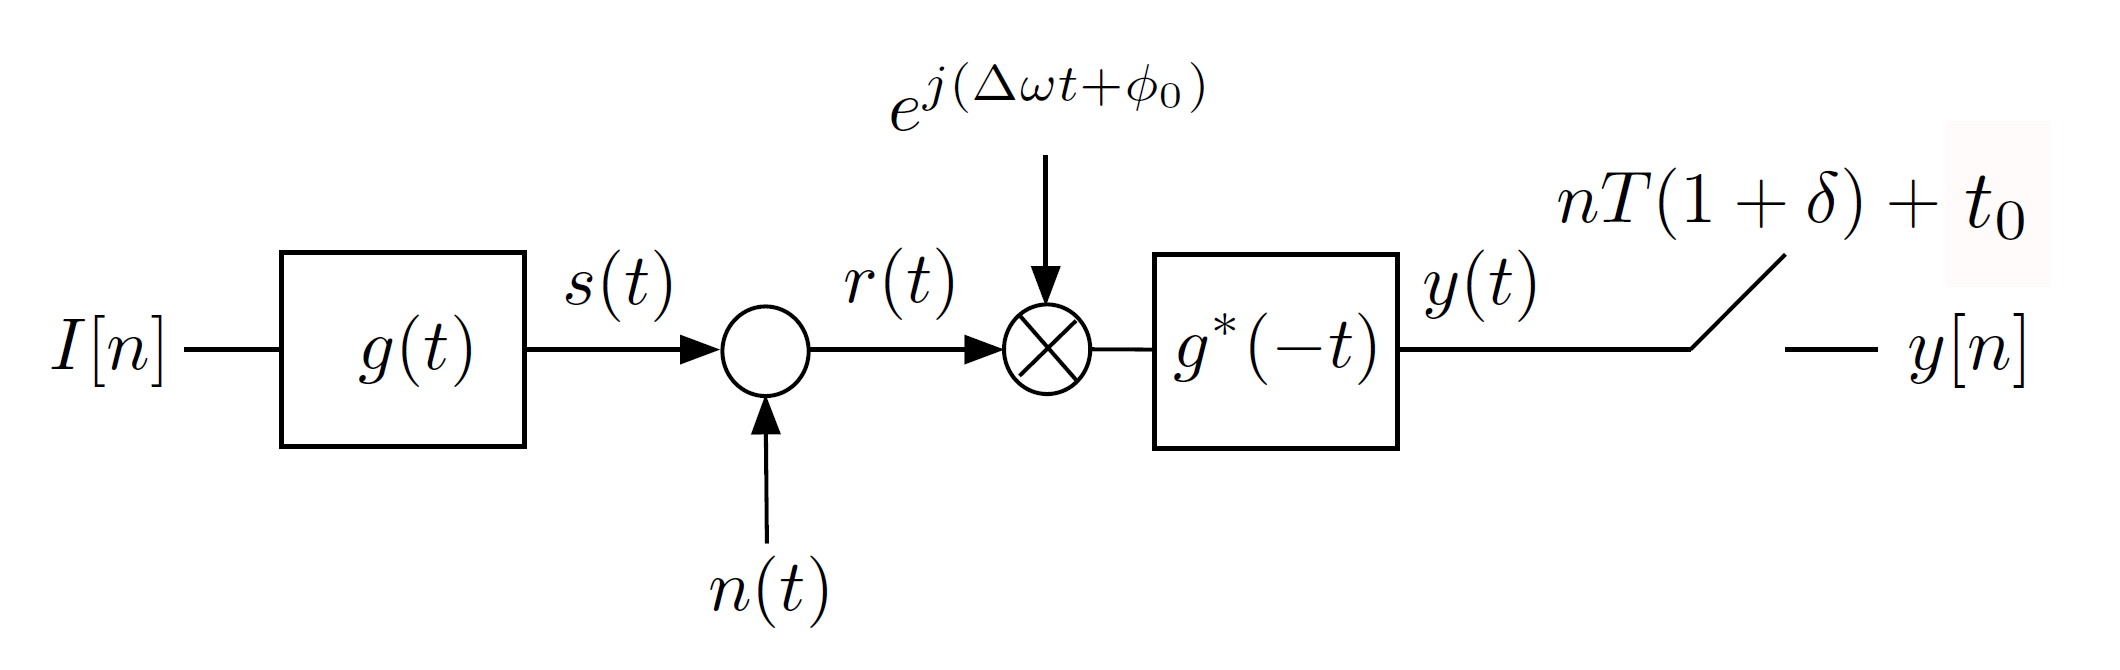
\includegraphics[width=0.8\linewidth]{Images/sync-errors-conceptual} 
		\caption{Synchronization mismatches at the receiver}
		\label{fig:sync-errors-conceptual}
	\end{figure}
	Accurate demodulation requires transmitter-receiver synchronization: precise symbol sampling instances and carrier frequency/phase alignment. Errors stem from independent local oscillators and propagation delay.
	\par
	Key synchronization errors:
	\begin{itemize}
		\item Carrier Frequency Offset (CFO), $\Delta f$: Difference between transmitter and receiver carrier frequencies.
		\item Carrier Phase Offset, $\phi_0$: Phase difference between incoming carrier and receiver local oscillator.
		\item Sample Clock Offset (SCO), $\delta$: Frequency mismatch between transmitter DAC clock and receiver ADC clock (neglected in this project).
		\item Sample Time Shift, $t_0$: Receiver uncertainty about symbol arrival time.
	\end{itemize}
	Figure \ref{fig:sync-errors-conceptual} illustrates these mismatches: symbols generated at $nT_{symb}$ are effectively sampled at $nT_{symb}(1+\delta)+t_0$ by the receiver.
	
	
	\subsection{Impact of Synchronization Errors on Performance}
	\subsubsection{Impact of Carrier Phase Offset ($\phi_0$)}
	A static carrier phase offset $\phi_0$ rotates the received constellation by $\phi_0$. With perfect timing, no CFO, and no noise, a transmitted symbol $I[n]$ becomes at the matched filter output:
	\begin{equation}
		y[n] = I[n]e^{j\phi_0}
	\end{equation}
	Uncorrected rotation causes detection errors. Figure \ref{fig:cfo-po-sub} illustrates the smearing of constellation points due to phase offset and CFO. The BER degradation from pure phase offset results in a performance floor or significant penalty depending on $\phi_0$'s magnitude.
	
	\subsubsection{Impact of Carrier Frequency Offset ($\Delta f$)}
	\begin{figure}[H]
		\centering
		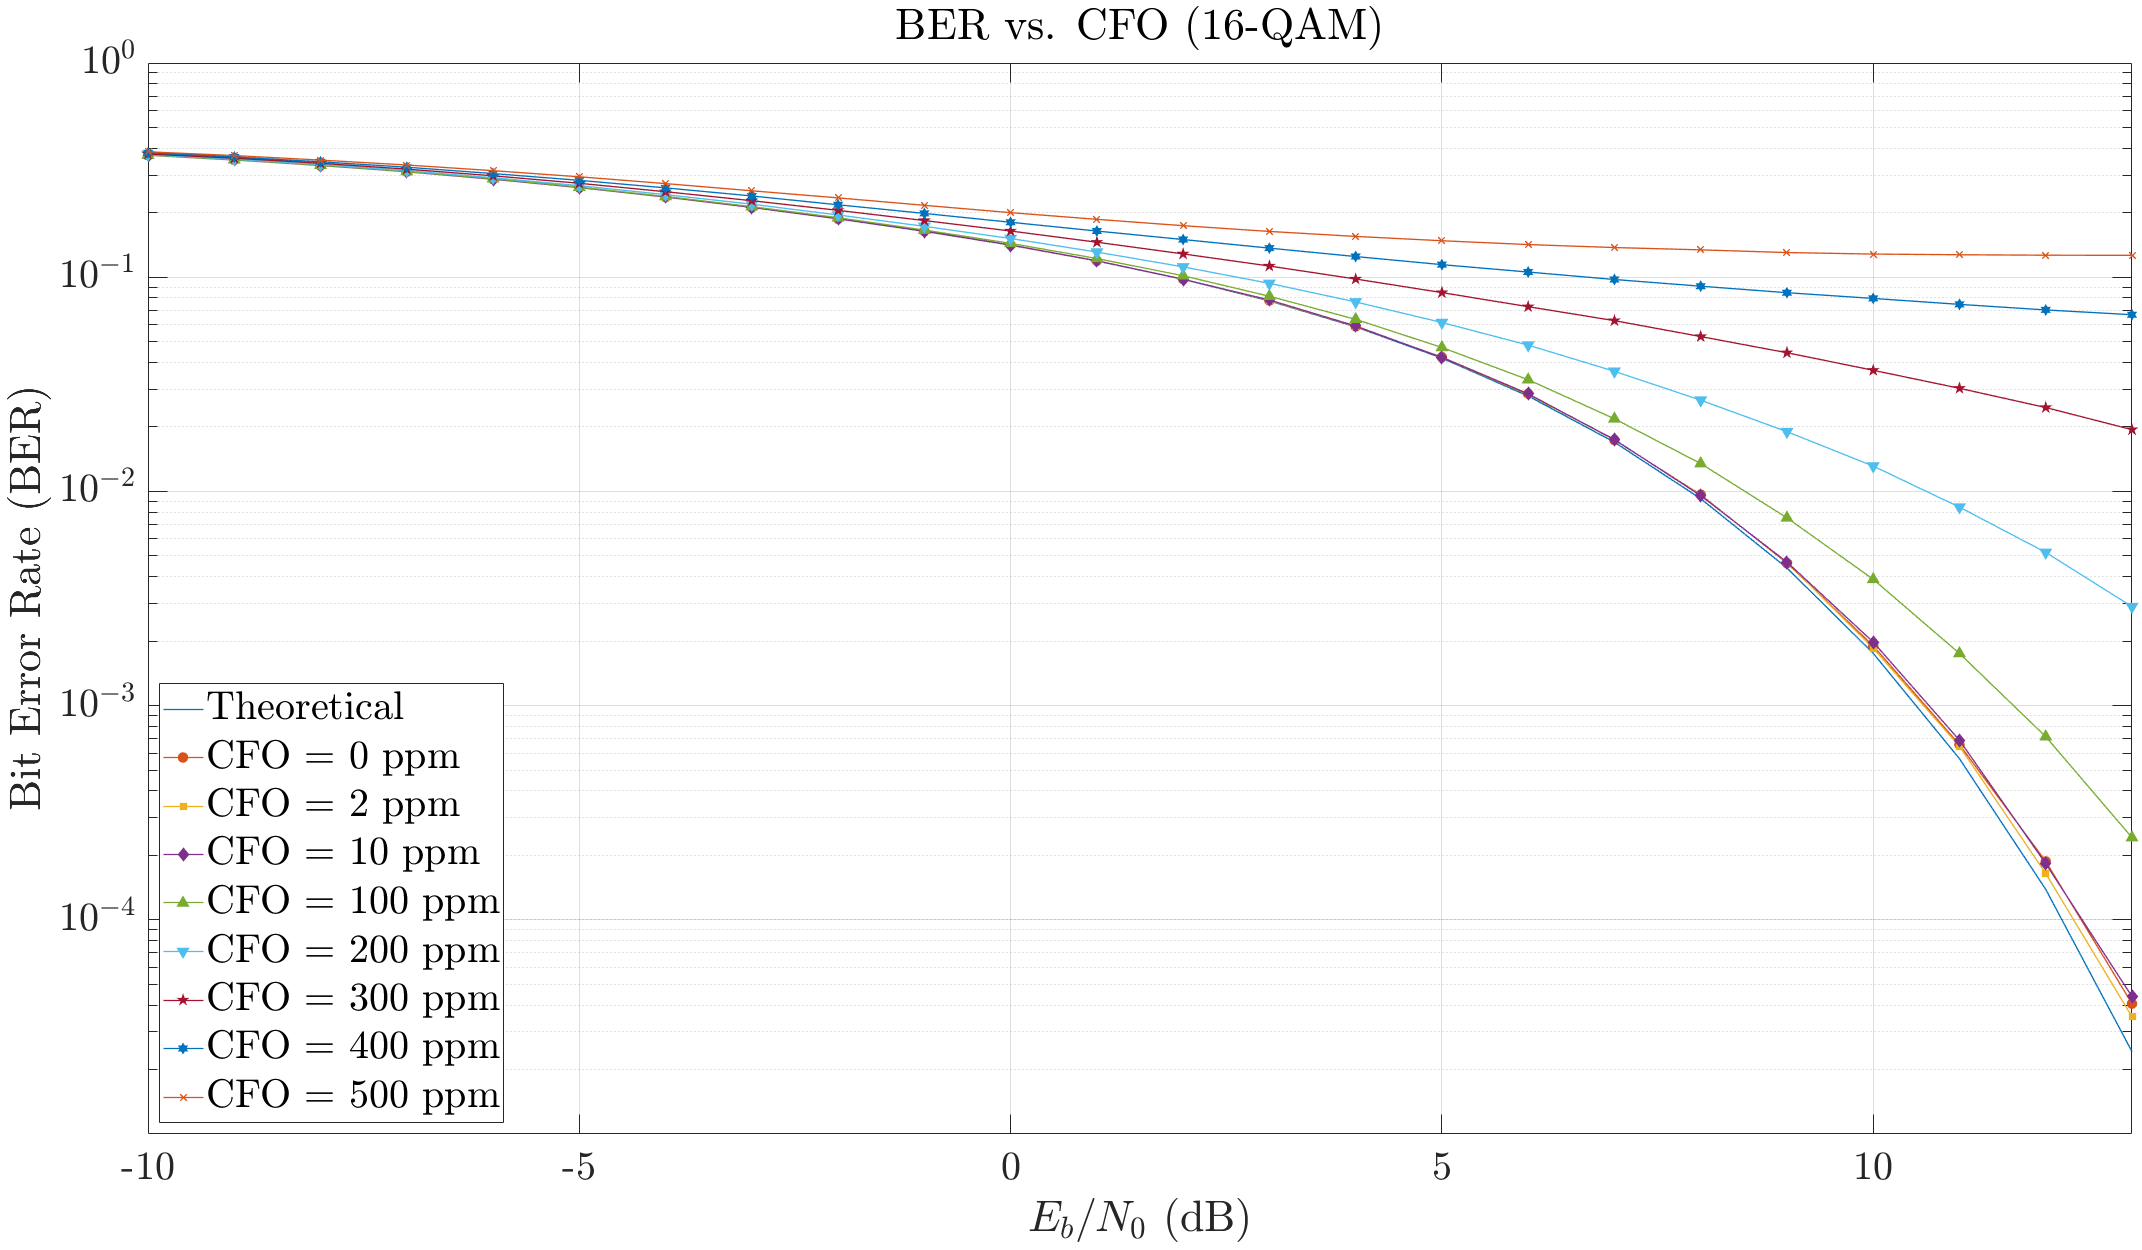
\includegraphics[width=0.8\linewidth]{Images/ber-cfo}
		\caption{Simulated BER vs. $E_b/N_0$ for 16-QAM with varying CFO, illustrating the ISI impact.}
		\label{fig:ber-cfo}
	\end{figure}
	With CFO $\Delta f$, the pre-matched filter signal is $r(t)e^{j(2\pi \Delta f t + \phi_0)}$. The impact of CFO is twofold:
	\begin{enumerate}
		\item Phase Drift: At the matched filter output, if CFO is uncompensated, sampled symbols $y[n] = I[n]e^{j(2\pi \Delta f nT_{symb} + \phi_0')}$ exhibit progressive phase rotation. This smears constellation points into arcs, as depicted in Figure \ref{fig:cfo-po-sub}.
		\item Inter-Symbol Interference (ISI): Significant CFO shifts the transmitted signal $s(t)$ spectrum. If uncorrected before the matched filter $g^*(-t)$, the filter is no longer matched to $g(t)e^{j2\pi \Delta f t}$. This mismatch causes SNR loss and introduces ISI because $h'(t) = (g(t)e^{j2\pi \Delta f t}) \otimes g^*(-t)$ no longer perfectly satisfies the Nyquist zero-ISI criterion. Figure \ref{fig:ber-cfo} quantifies this BER degradation for 16-QAM under different CFO values. A CFO of 50-100 ppm leads to a significant $E_b/N_0$ penalty or an error floor.
	\end{enumerate}
	
	\subsubsection{Impact of Sample Time Shift ($t_0$)}
	\begin{figure}[H]
		\centering
		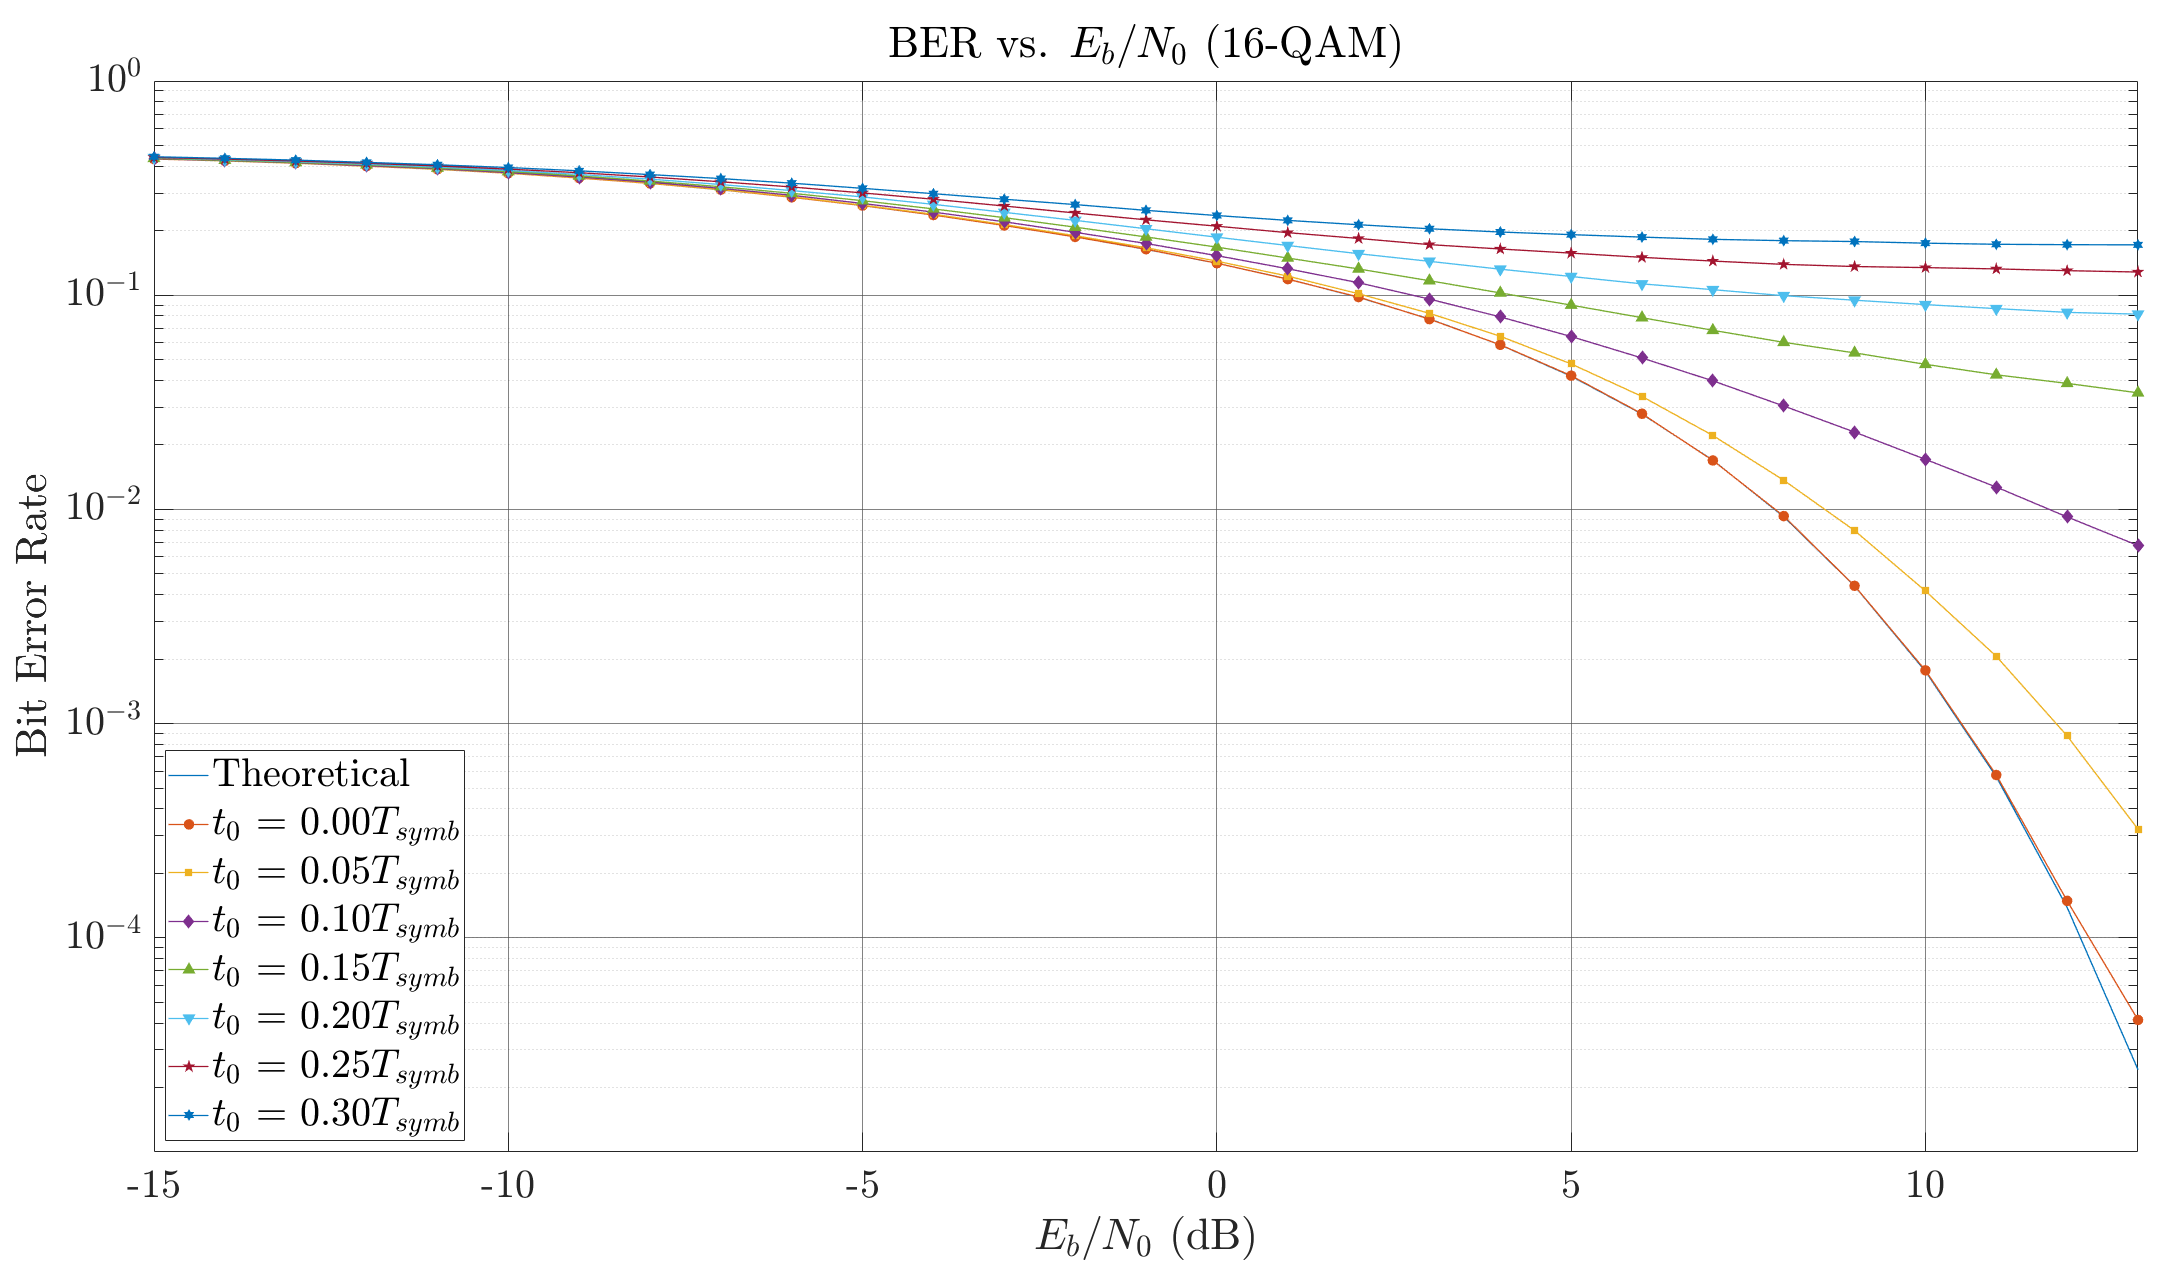
\includegraphics[width=0.8\linewidth]{Images/ber-timing}
		\caption{Simulated BER vs. $E_b/N_0$ for 16-QAM with varying timing offsets $t_0/T_{symb}$.}
		\label{fig:ber-timing}
	\end{figure}
	An incorrect sampling instant $t_0 \neq 0$ means sampling the matched filter output $h(t)$ at $nT_{symb} + t_0$. The received sample, sans noise, is:
	\begin{align}
		y[n] &= \sum_m I[m]h((n-m)T_{symb} + t_0) \\
		&= I[n]h(t_0) + \sum_{m \neq n} I[m]h((n-m)T_{symb} + t_0) \label{eq:timing_offset_impact_revised_style_change}
	\end{align}
	The term $I[n]h(t_0)$ is the attenuated symbol ($h(t_0) < h(0)$ for $t_0 \neq 0$). The sum is ISI ($h(kT_{symb} + t_0) \neq 0$ for $k \neq 0, t_0 \neq 0$). Figure \ref{fig:ber-timing} shows BER degradation for 16-QAM with increasing $t_0$. Fractional deviations like $0.1 T_{symb}$ to $0.2 T_{symb}$ cause severe performance loss. Figure \ref{fig:cfo-po-to-sub} visually shows the combined detrimental effects of CFO, phase offset, and timing offset.
	
	\begin{figure}[H]
		\centering
		\begin{subfigure}[b]{0.48\textwidth}
			\centering
			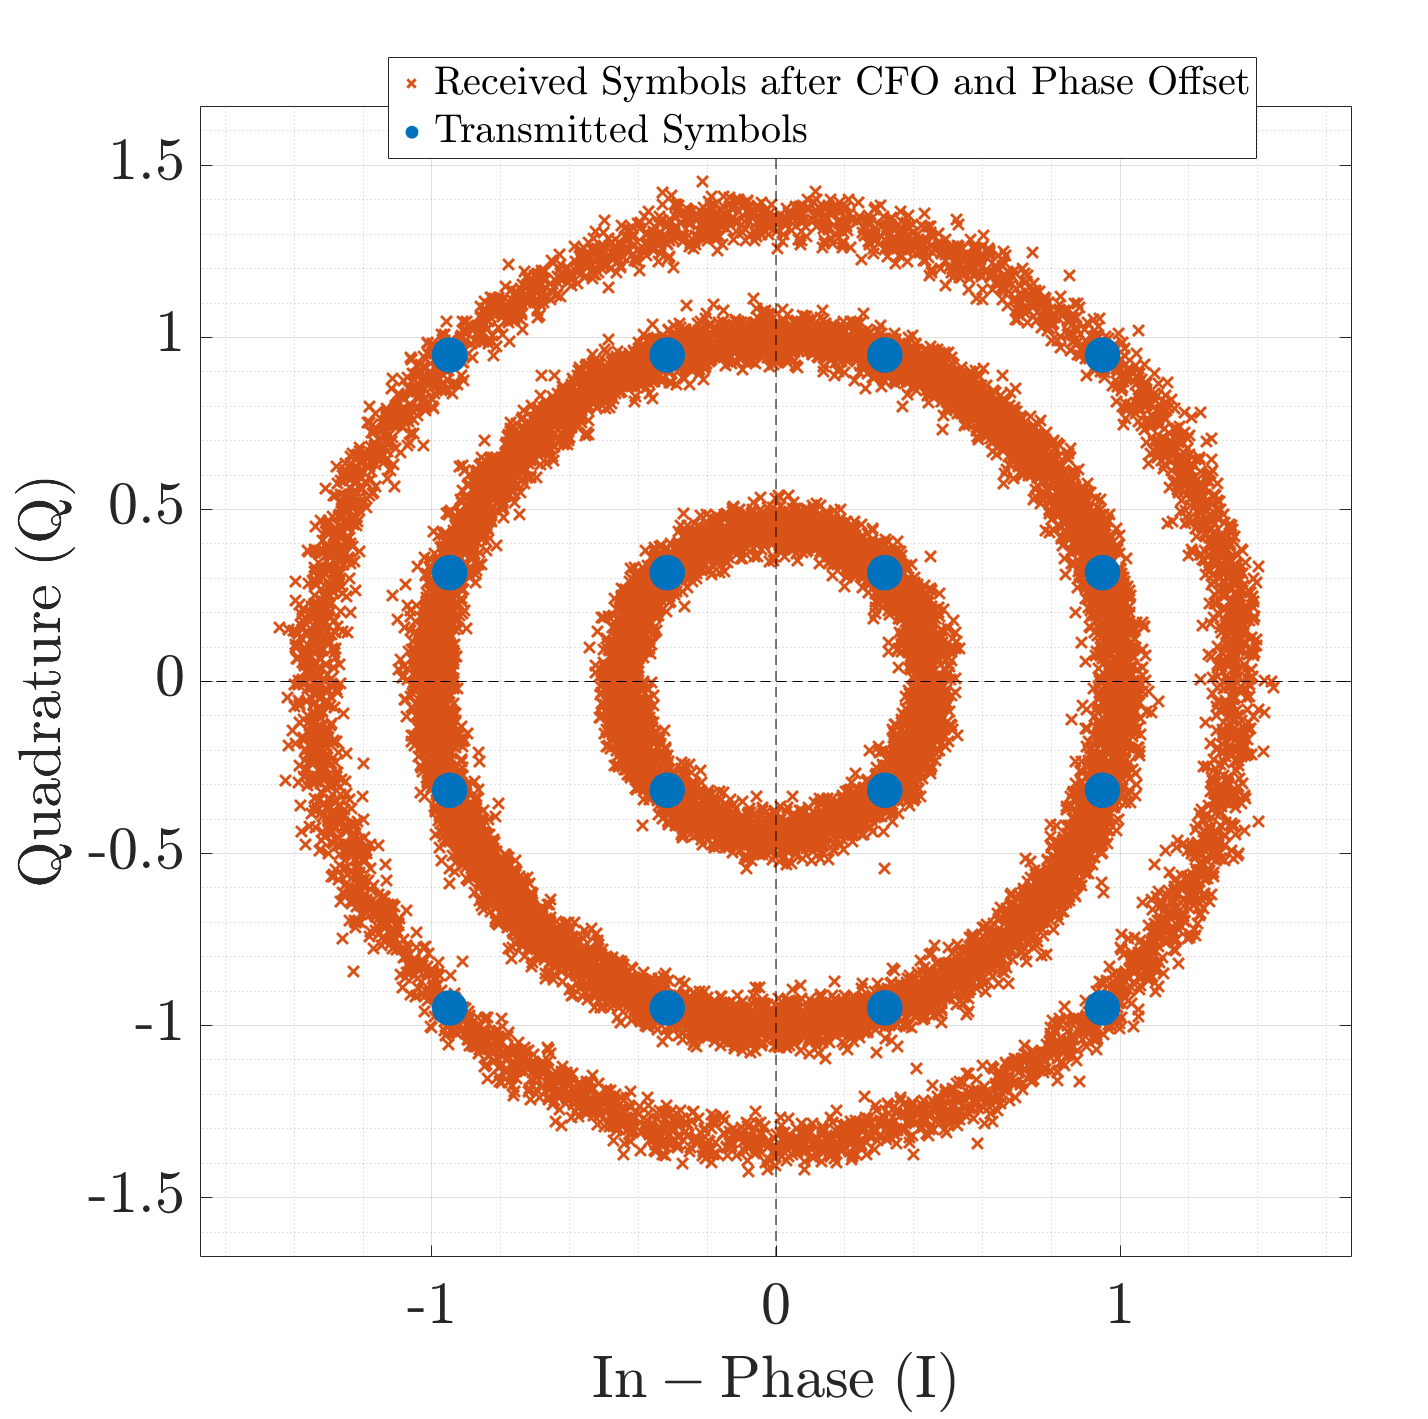
\includegraphics[width=\linewidth]{Images/cfo-po}
			\caption{16-QAM Constellation after CFO (20 ppm) and Phase Offset ($\pi/8$). $E_b/N_0 = 20$ dB.}
			\label{fig:cfo-po-sub}
		\end{subfigure}
		\hfill  
		\begin{subfigure}[b]{0.48\textwidth}
			\centering
			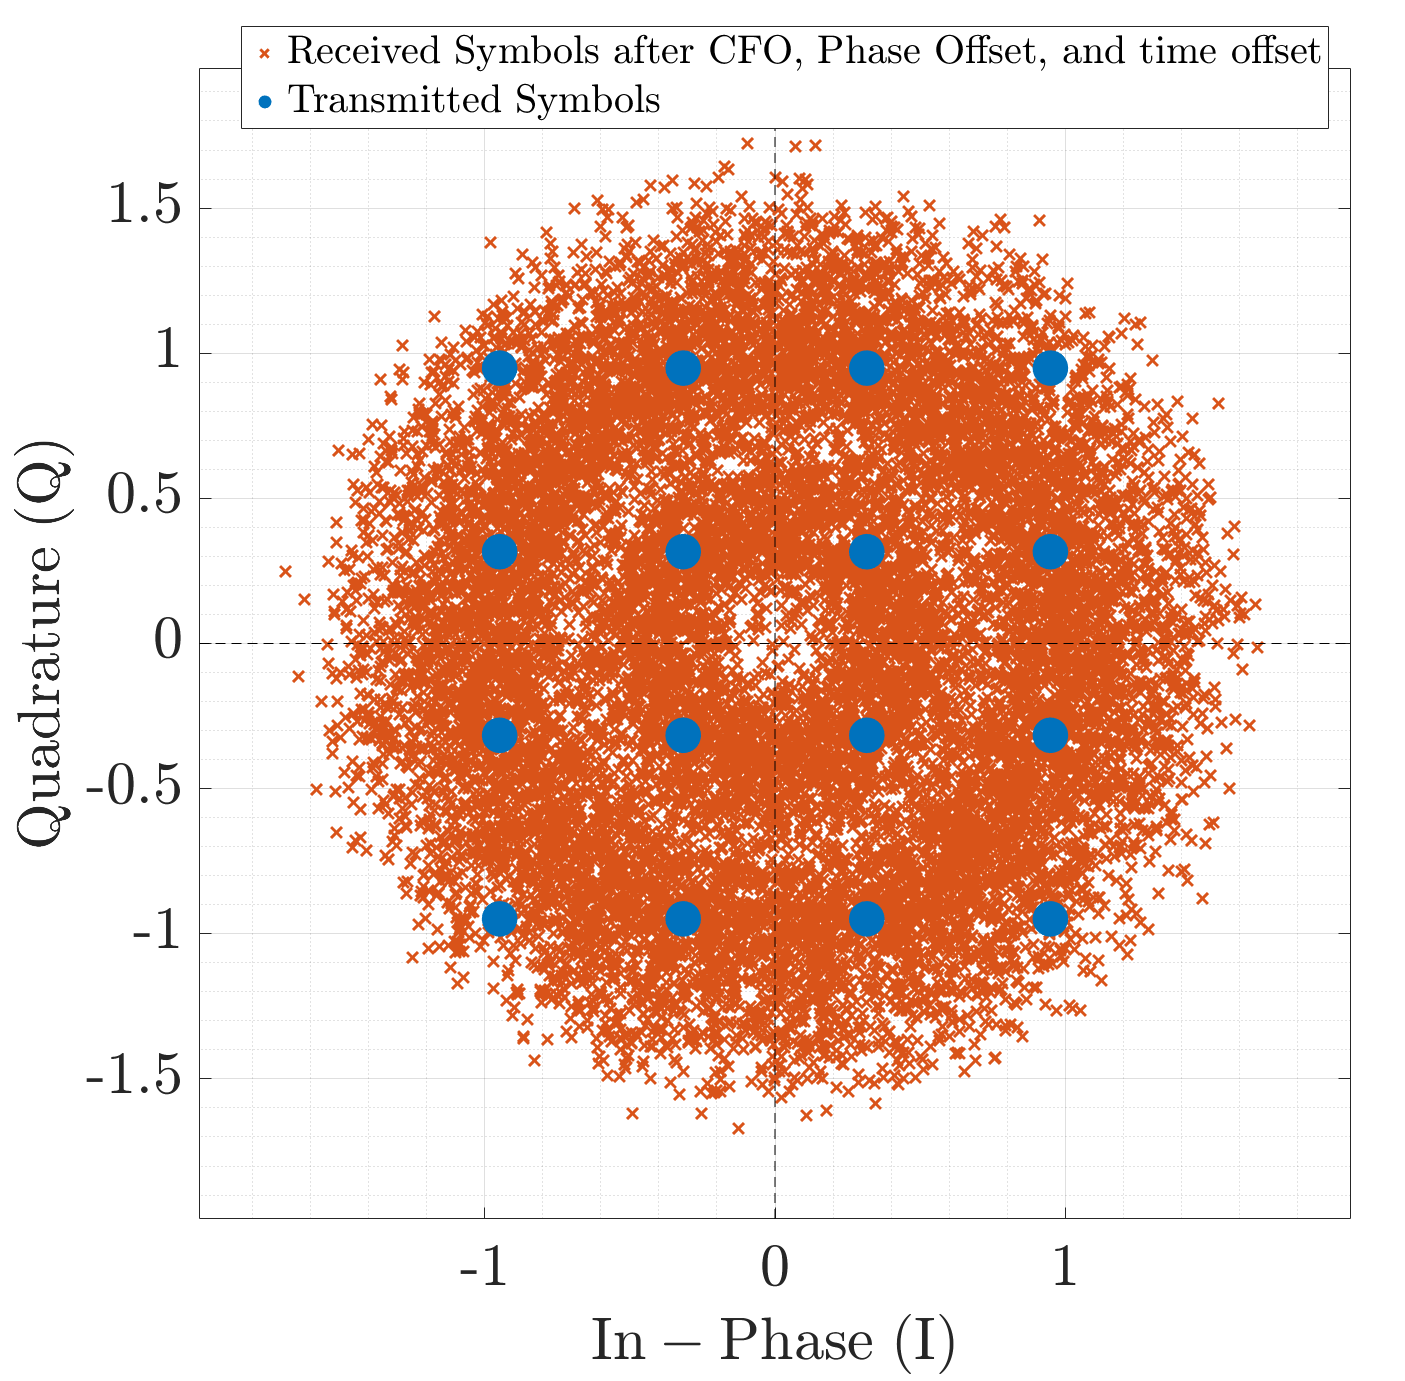
\includegraphics[width=\linewidth]{Images/cfo-po-to}
			\caption{16-QAM Constellation after CFO (20 ppm), Phase Offset ($\pi/8$) and time offset ($t_0 = 0.1 T_{symb}$). $E_b/N_0 = 20$ dB.}
			\label{fig:cfo-po-to-sub}
		\end{subfigure}
		\caption{Simulated Constellation diagrams: impact of synchronization errors on 16-QAM.}
		\label{fig:cfo-combined_style_change}
	\end{figure}
	
	\subsection{Gardner Algorithm for Timing Recovery}
	The Gardner algorithm is a non-data-aided (NDA) feedback algorithm correcting sampling time errors. It estimates and corrects the normalized time shift $\epsilon[n]$ progressively.
	
	\paragraph{Principle:}
	The algorithm observes samples at symbol instants and midway between them. The timing estimate $\hat{\epsilon}[n]$ update equation at symbol time $n$ is:
	\begin{equation}
		\hat{\epsilon}[n+1] = \hat{\epsilon}[n] - \kappa \cdot \text{Re} \left\{ y_{\hat{\epsilon}[n]}[n-1/2] \left( y_{\hat{\epsilon}[n]}^{*}[n] - y_{\hat{\epsilon}[n-1]}^{*}[n-1] \right) \right\}
		\label{eq:gardner_update_style_change}
	\end{equation}
	where:
	\begin{itemize}
		\item $\hat{\epsilon}[n]$ is the current normalized time error estimate.
		\item $\kappa$ is the loop gain (error weight), controlling convergence and stability.
		\item $y_{\hat{\epsilon}[n]}[n]$ is the sample at the estimated correct timing for symbol $n$.
		\item $y_{\hat{\epsilon}[n]}[n-1/2]$ is the sample midway between estimated correct timings for symbols $n-1$ and $n$.
		\item $(y_{\hat{\epsilon}[n]}^{*}[n] - y_{\hat{\epsilon}[n-1]}^{*}[n-1])$ approximates the signal slope.
	\end{itemize}
	The algorithm requires two input samples per symbol. The error term's sign indicates shift direction; its magnitude indicates extent.
	
	\paragraph{Performance and Convergence:}
	Figure \ref{fig:gardner1} illustrates the mean time error $\hat{\epsilon}[n]$ convergence to the true time shift for various loop gains $\kappa$. Smaller $\kappa$ yields slower convergence but less steady-state jitter; larger $\kappa$ speeds convergence but increases jitter or causes instability.
	
	The Gardner algorithm is robust to CFO and phase offsets. Figure \ref{fig:gardner2} demonstrates this robustness, showing convergence under various CFO conditions. Performance remains stable for typical CFO values.
	
	\begin{figure}[H]
		\centering
		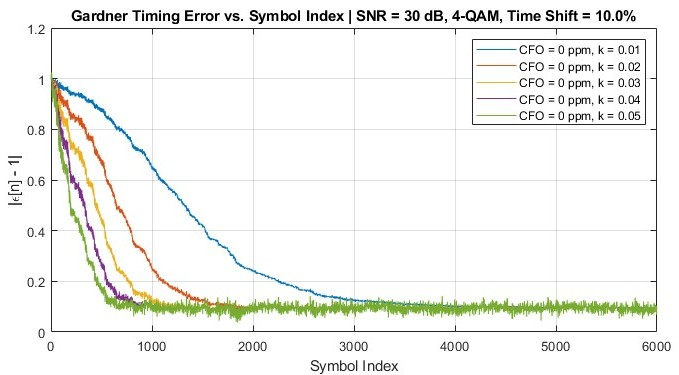
\includegraphics[width=0.7\linewidth]{Images/Gardner_k_list.jpg} 
		\caption{Simulated Gardner algorithm time error estimate convergence for different loop gain values ($\kappa$). The plot shows mean estimated time error vs. symbol number, converging to the applied time shift.}
		\label{fig:gardner1}
	\end{figure}
	
	\begin{figure}[H]
		\centering
		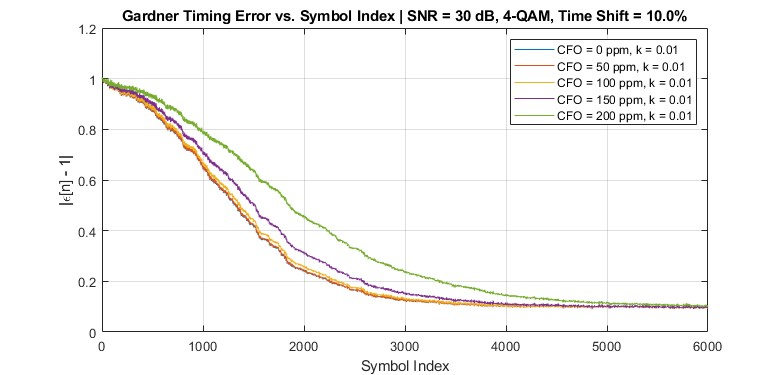
\includegraphics[width=0.7\linewidth]{Images/Gardner_CFO_robust.jpg} 
		\caption{Simulated Gardner algorithm robustness to Carrier Frequency Offset (CFO). The plot shows time error estimate convergence for a fixed $\kappa$ under different CFOs, demonstrating minimal impact.}
		\label{fig:gardner2}
	\end{figure}
	
	\subsection{Frame and Frequency Acquisition}
	After timing recovery, frame synchronization (detecting pilot sequence start) and coarse CFO acquisition use a differential cross-correlator.
	
	\paragraph{Principle using Differential Cross-Correlator:}
	This data-aided (DA) method uses known pilot symbols $a[l]$. The differential cross-correlator output metric $D_k[n]$ is:
	\begin{equation}
		D_k[n] = \frac{1}{N_p-k} \sum_{l=k}^{N_p-1} (y^*[n+l]a[l])(y^*[n+l-k]a[l-k])^*
		\label{eq:diff_corr_metric_style_change}
	\end{equation}
	where $y[n]$ is the received sequence (post-Gardner), $a[l]$ is the pilot sequence of length $N_p$, and $k$ is a time shift. This metric multiplies two time-shifted windows of the pilot-received signal correlation.
	
	Pilot start position $\hat{n}$ (frame sync) is estimated by maximizing summed $|D_k[n]|$ over $k \in [1, K_{avg}]$:
	\begin{equation}
		\hat{n} = \text{arg max}_n \sum_{k=1}^{K_{avg}} |D_k[n]|
		\label{eq:frame_sync_est_style_change}
	\end{equation}
	
	CFO $\hat{\Delta f}$ is then estimated from $D_k[\hat{n}]$ phase at $\hat{n}$:
	\begin{equation}
		\hat{\Delta f} = -\frac{1}{K_{avg}} \sum_{k=1}^{K_{avg}} \frac{\angle D_k[\hat{n}]}{2\pi k T_{symb}}
		\label{eq:cfo_est_diff_corr_style_change}
	\end{equation}
	The differential nature provides CFO robustness.
	
	\paragraph{Performance Metrics:}
	Performance is evaluated by estimation error variance for $\hat{n}$ and $\hat{\Delta f}$ versus $E_b/N_0$, pilot length $N_p$, and averaging window $K_{avg}$.
	
	\begin{figure}[H]
		\centering
		\begin{subfigure}[b]{0.48\textwidth}
			\centering
			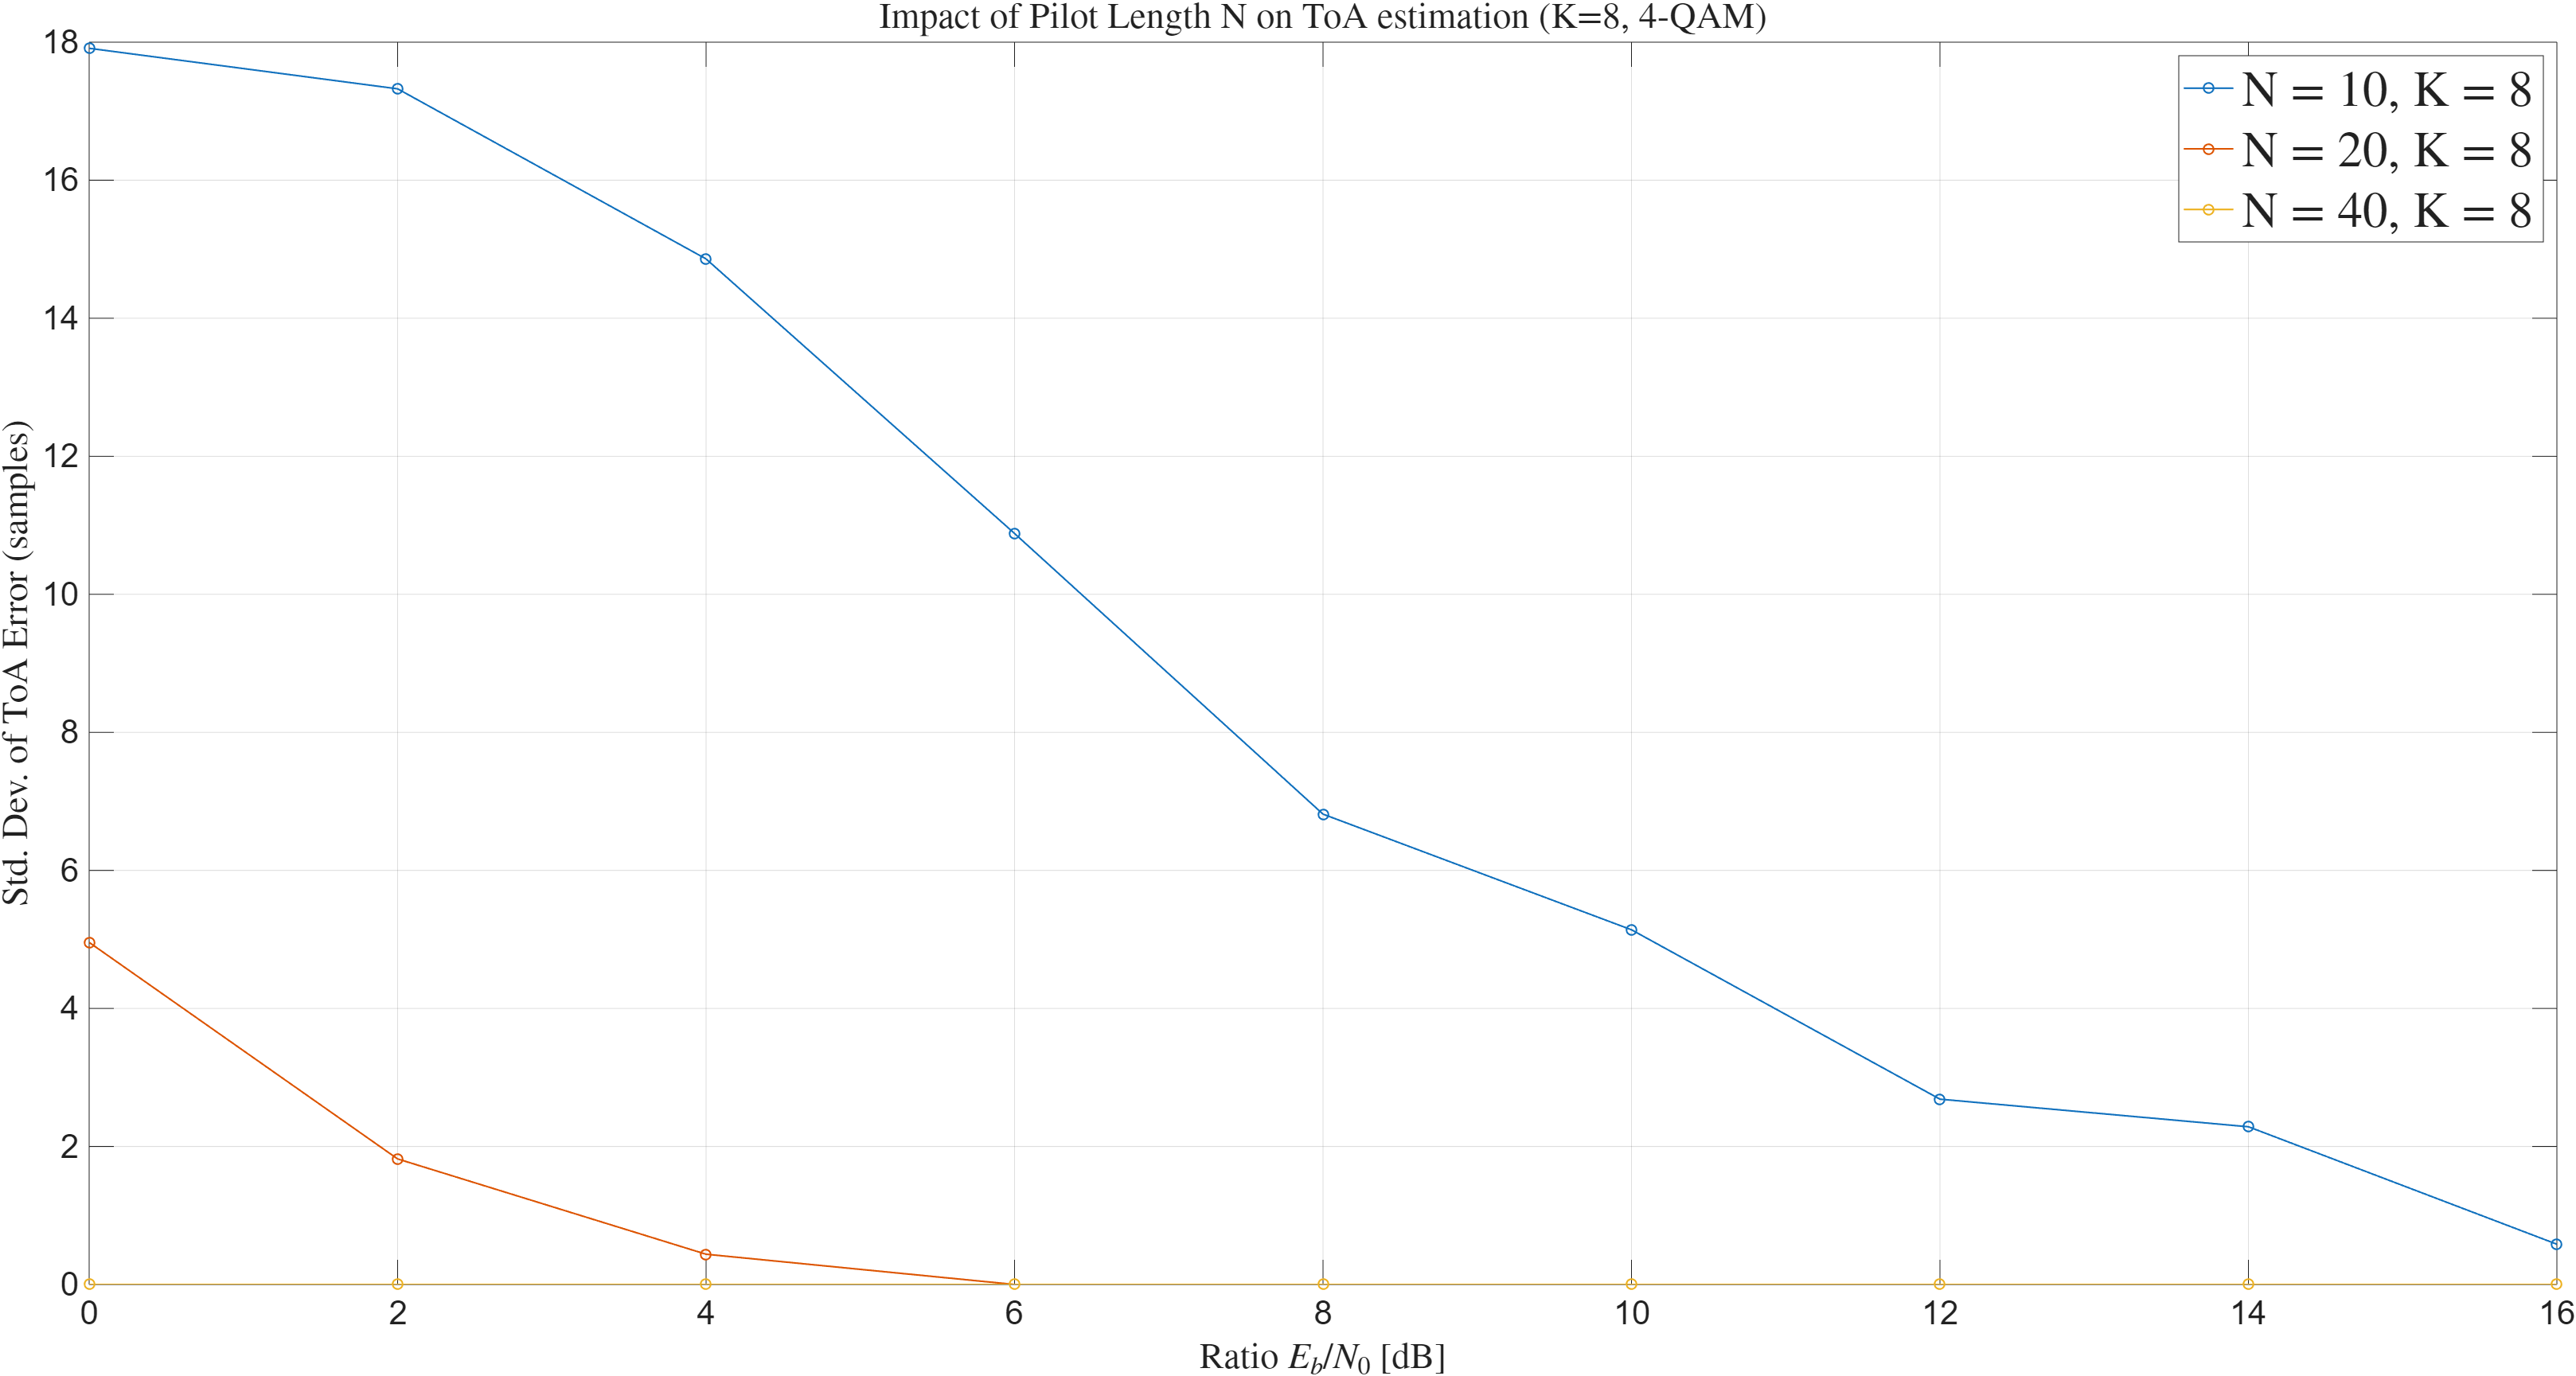
\includegraphics[width=\linewidth]{Images/frame_sync_pilot_len.png} 
			\caption{ToA error std dev vs. $E_b/N_0$.}
			\label{fig:frame_sync_pilot_len_style_change}
		\end{subfigure}
		\hfill
		\begin{subfigure}[b]{0.48\textwidth}
			\centering
			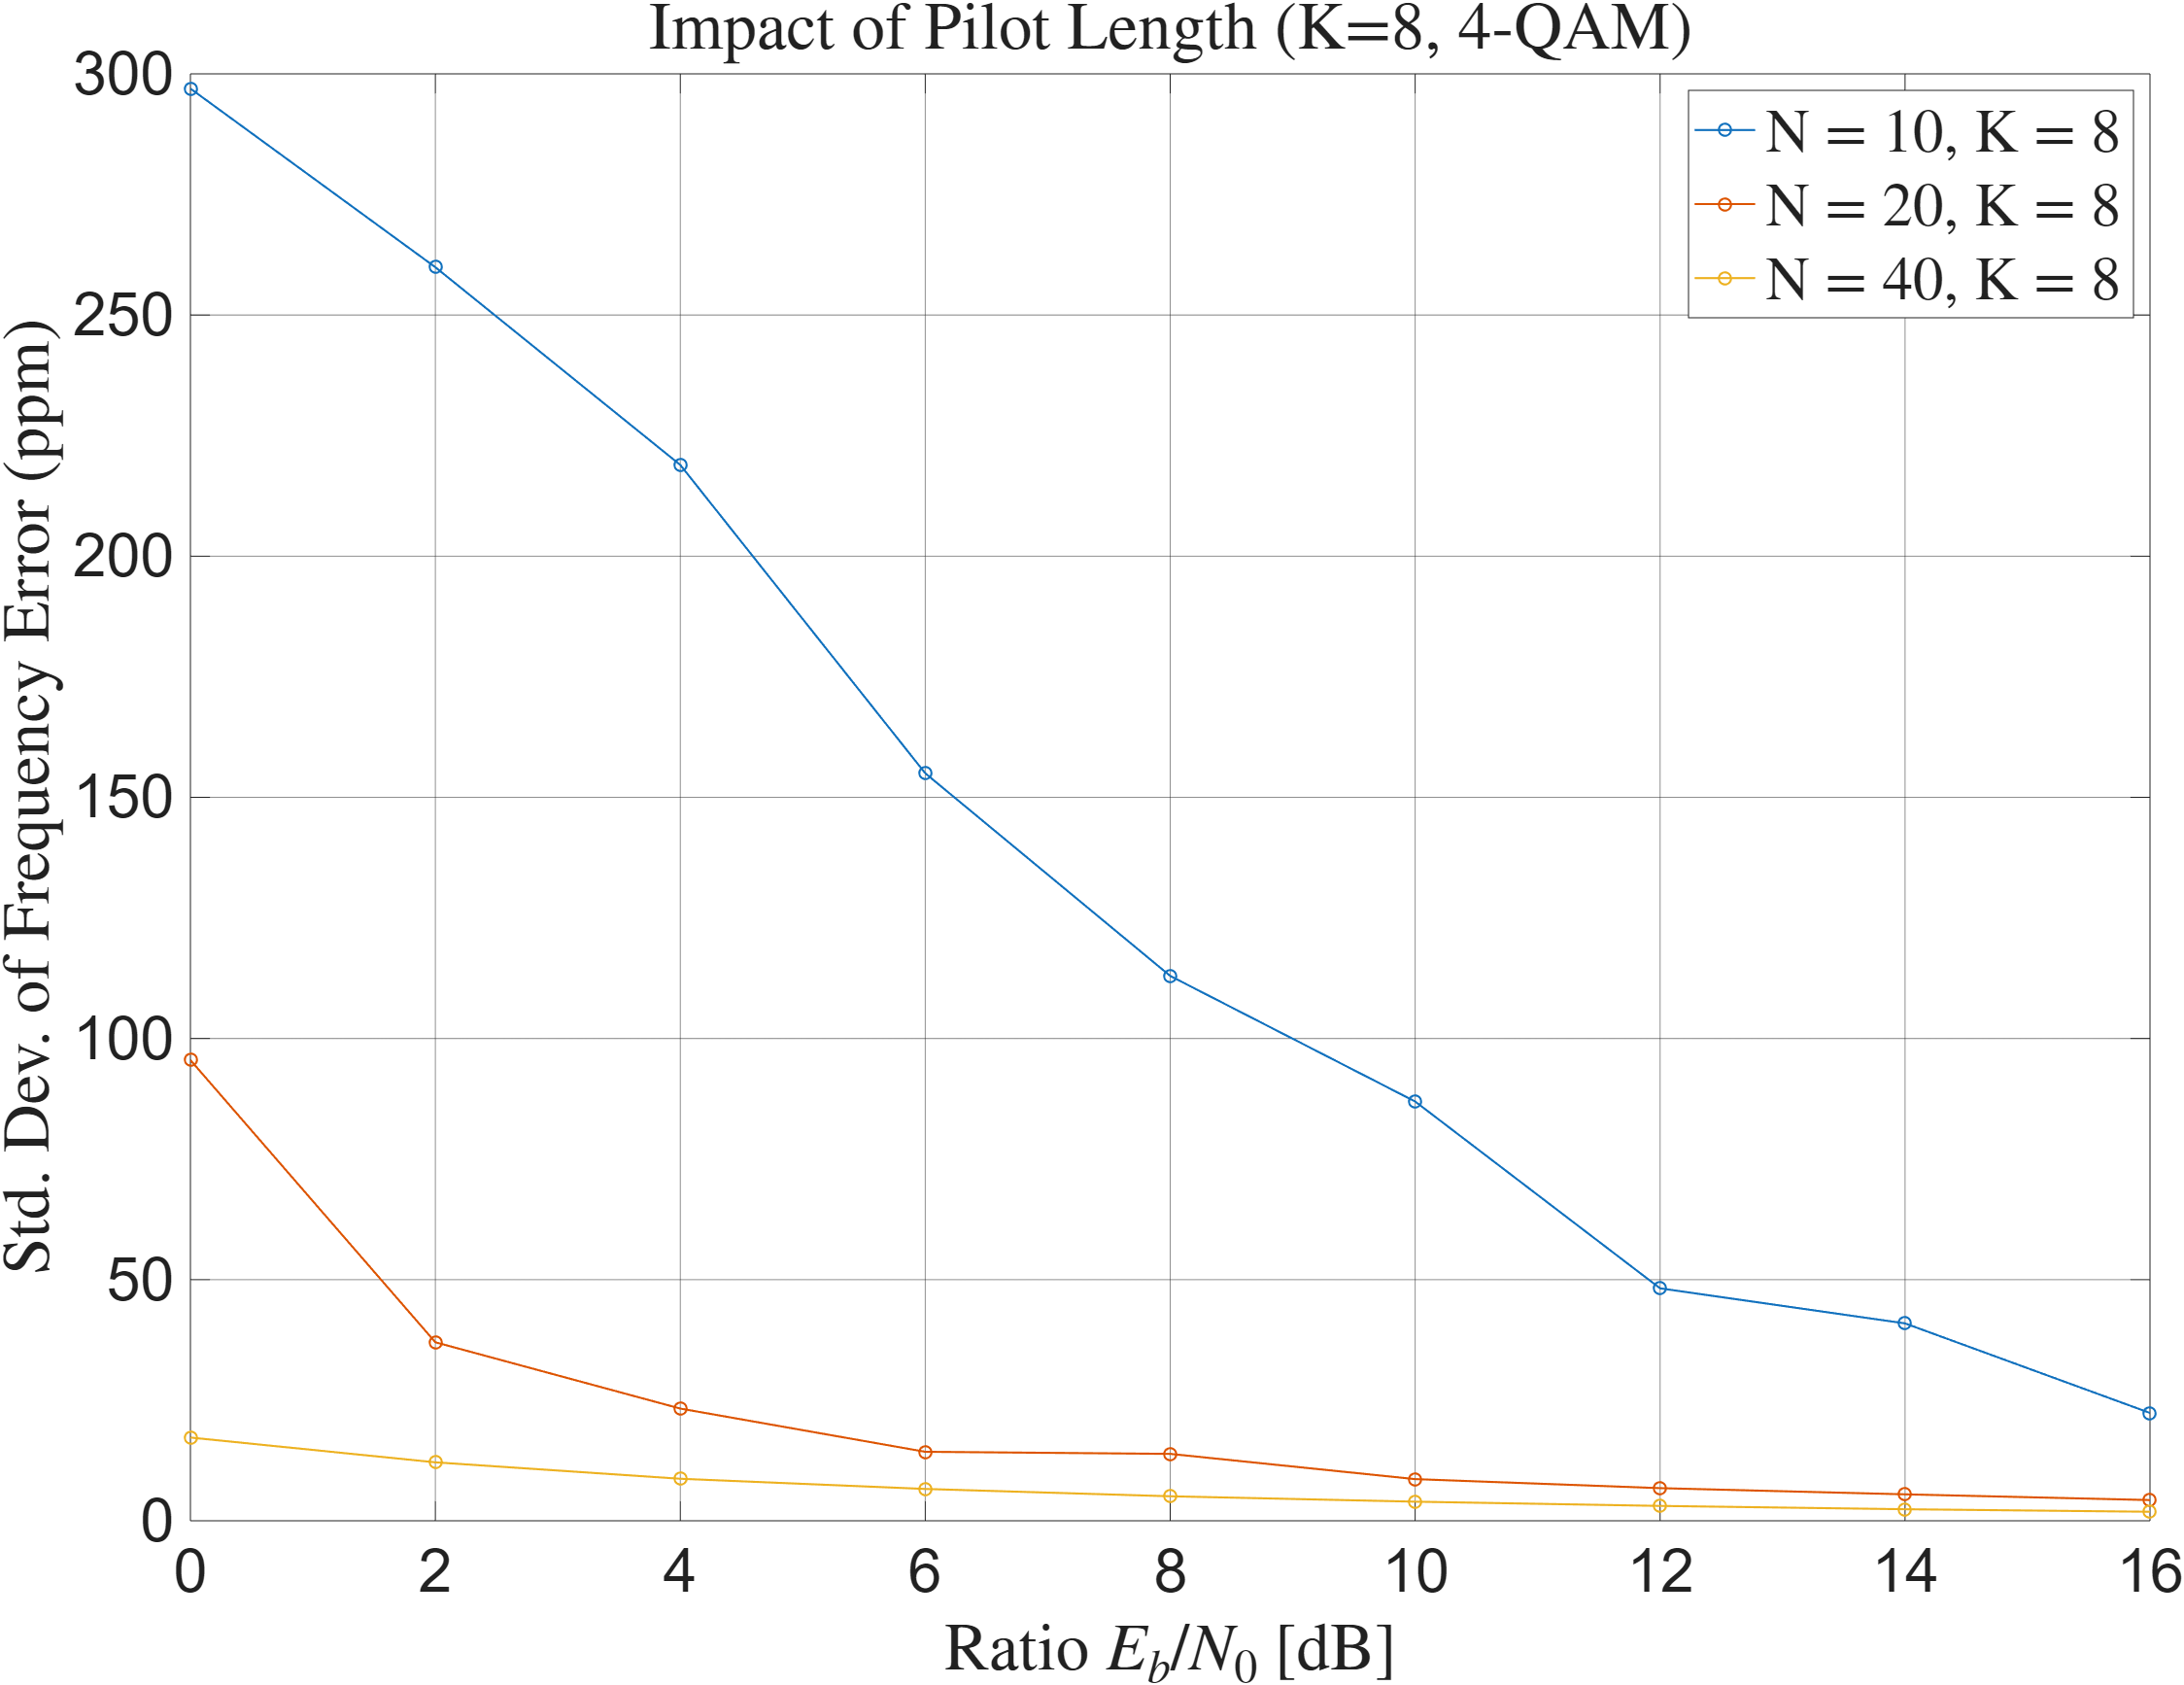
\includegraphics[width=\linewidth]{Images/cfo_est_pilot_len.png} 
			\caption{CFO error std dev vs. $E_b/N_0$.}
			\label{fig:cfo_est_pilot_len_style_change}
		\end{subfigure}
		\caption{Simulated standard deviation of Time-of-Arrival (ToA) and CFO estimation error vs. $E_b/N_0$ for different pilot sequence lengths ($N_p$). Longer pilots reduce error variance.}
		\label{fig:acquisition_vs_pilot_len}
	\end{figure}
	
	\begin{figure}[H]
		\centering
		\begin{subfigure}[b]{0.48\textwidth}
			\centering
			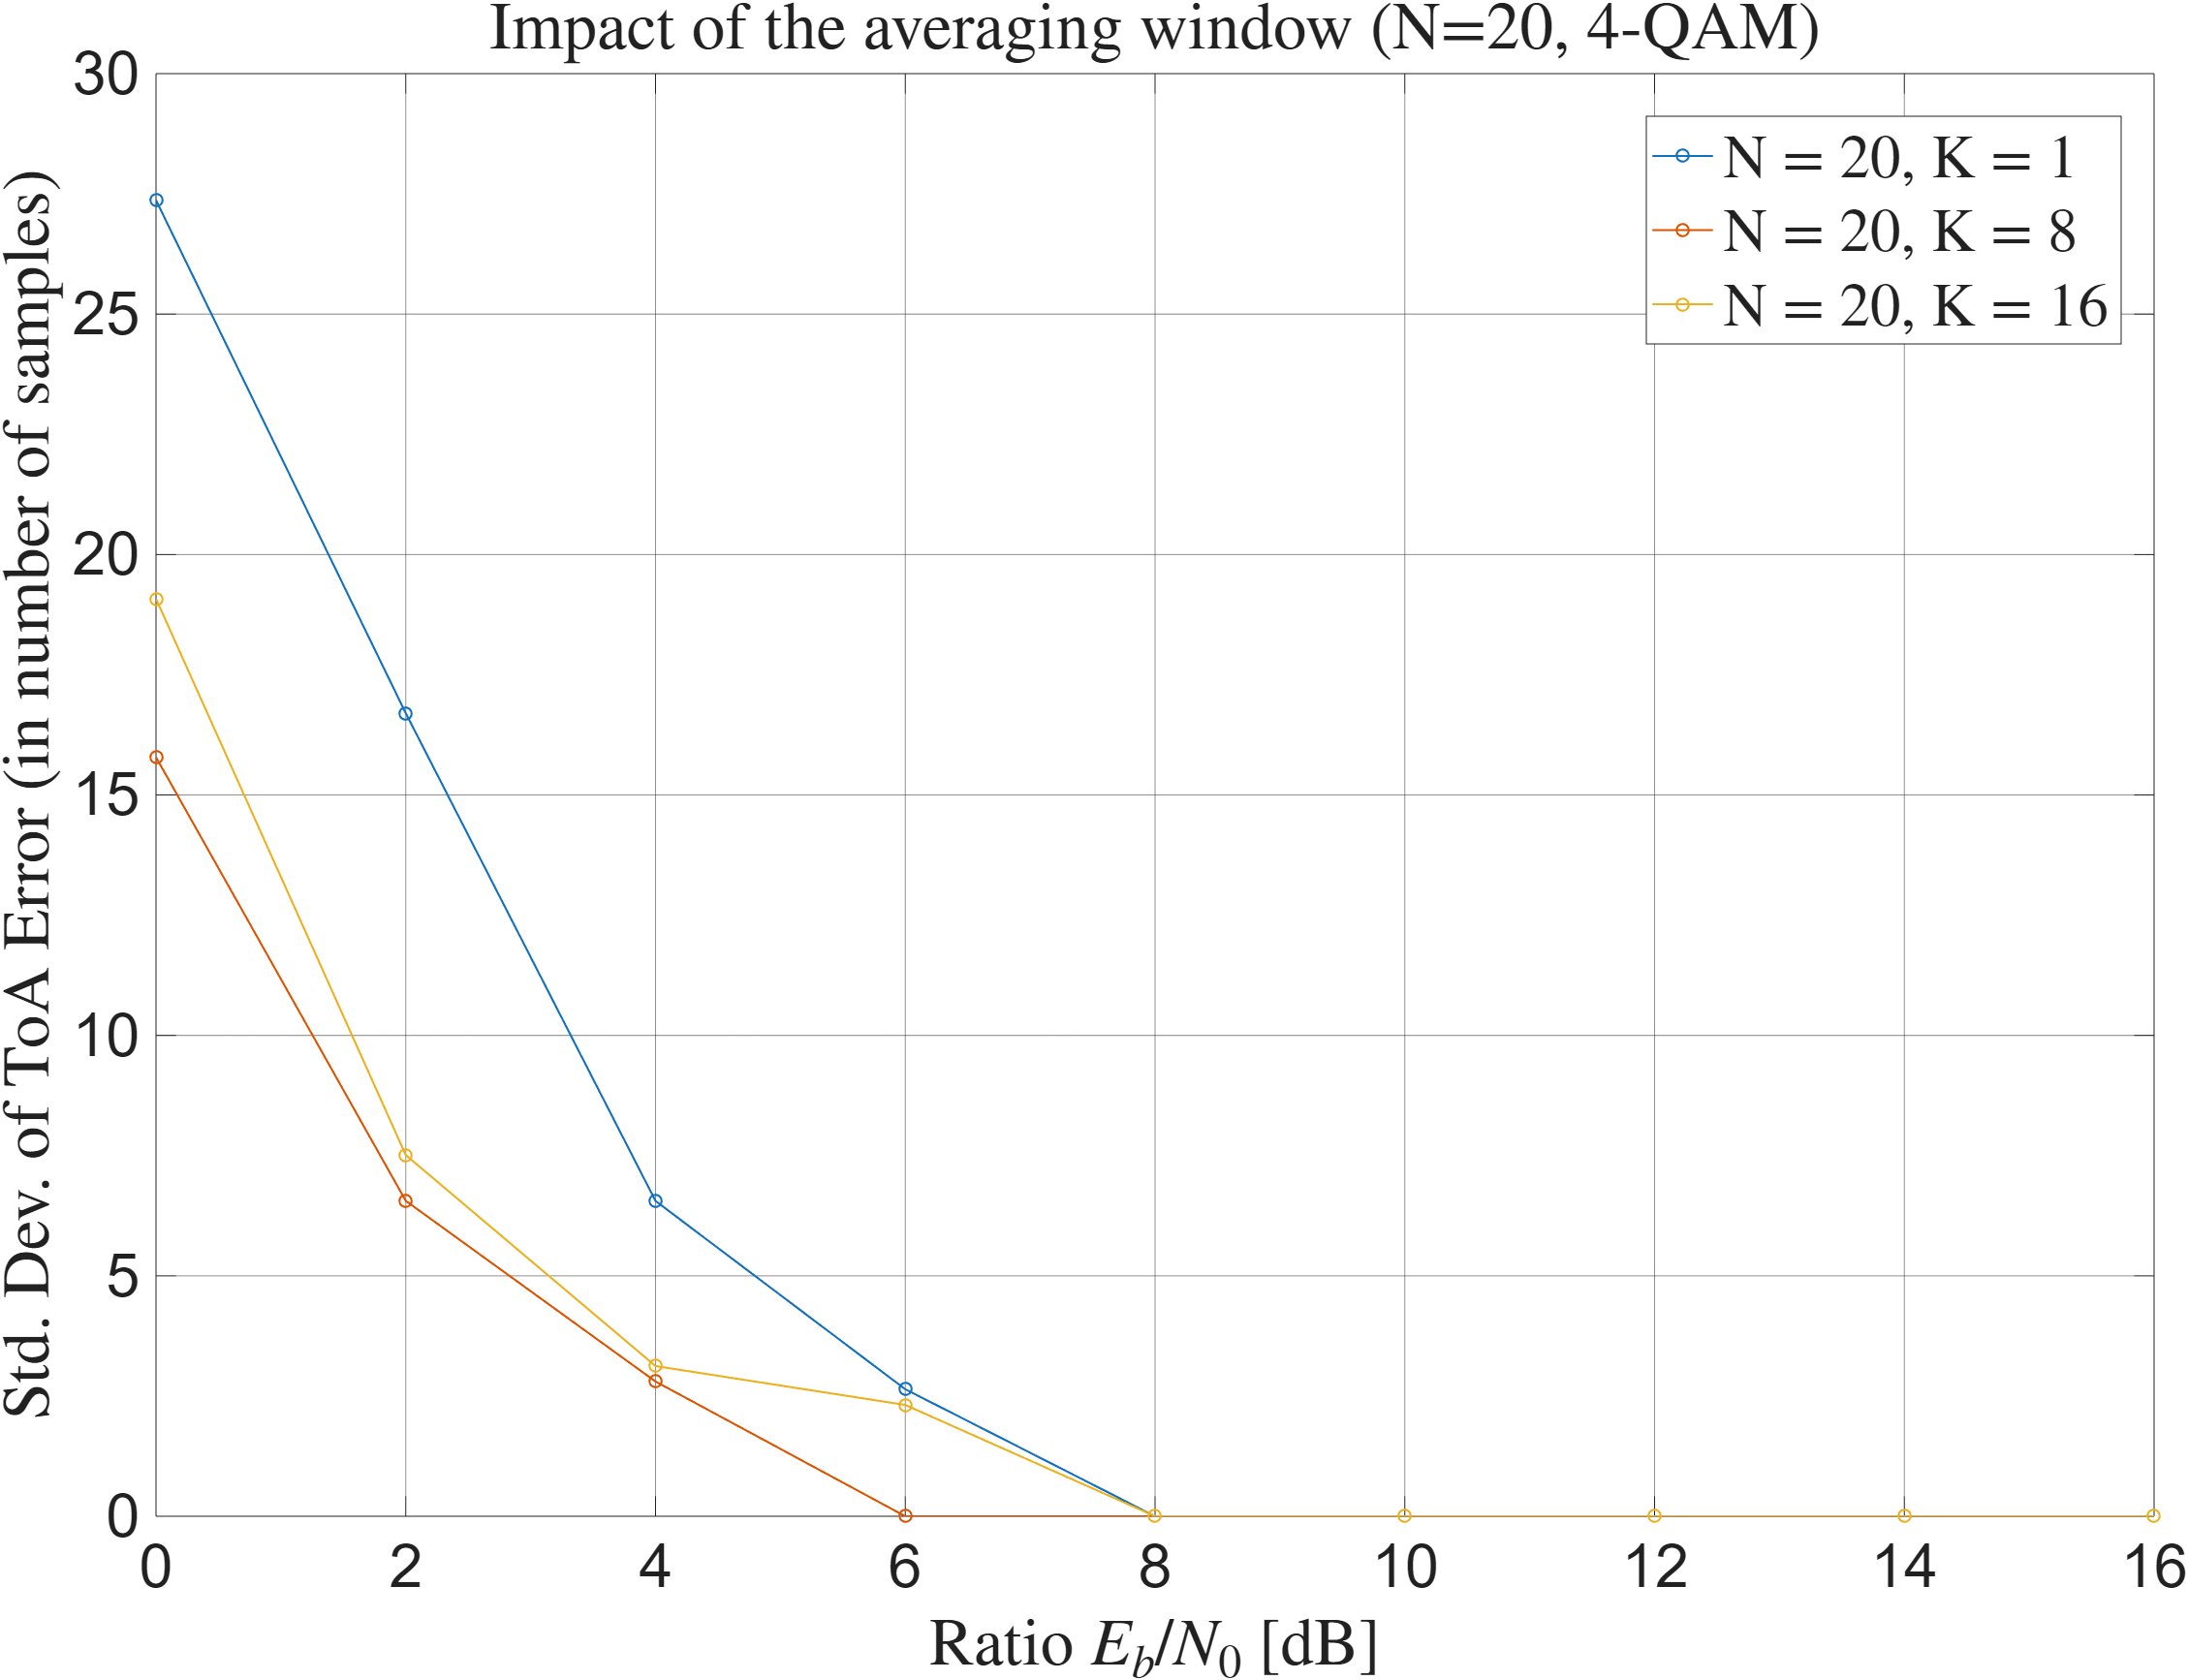
\includegraphics[width=\linewidth]{Images/frame_sync_K_avg.png} 
			\caption{ToA error std dev vs. $E_b/N_0$.}
			\label{fig:frame_sync_K_avg_style_change}
		\end{subfigure}
		\hfill
		\begin{subfigure}[b]{0.48\textwidth}
			\centering
			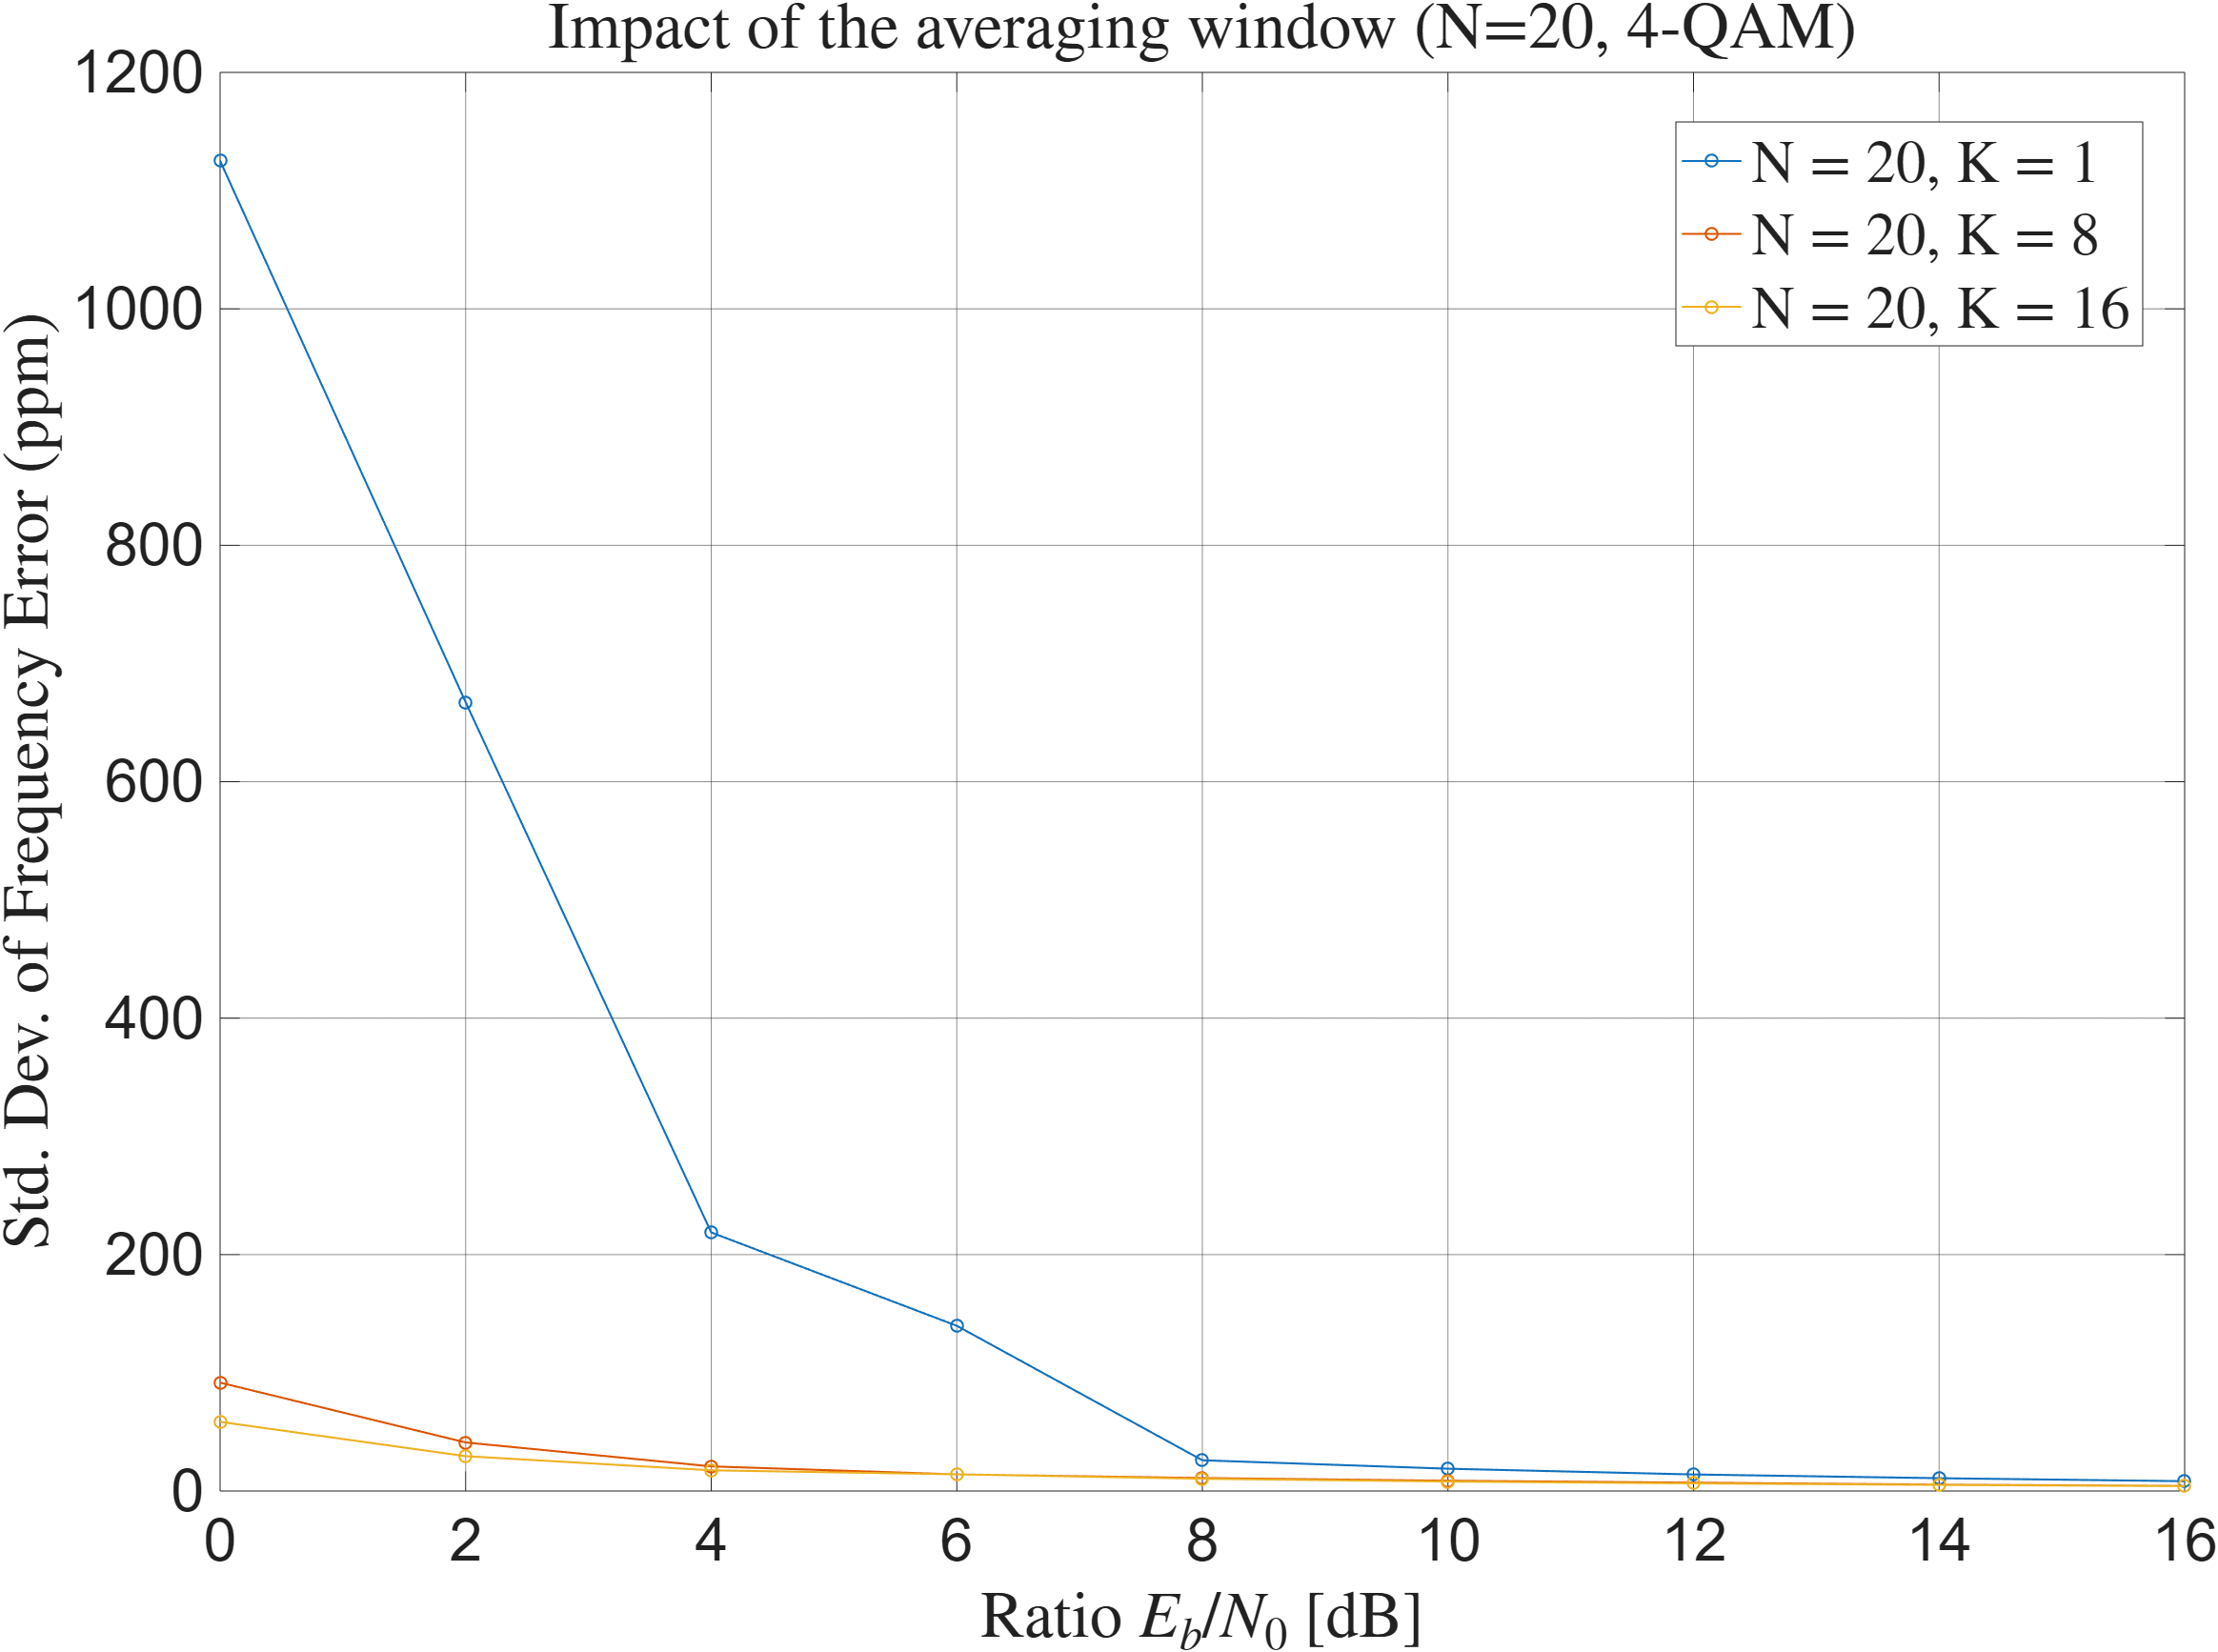
\includegraphics[width=\linewidth]{Images/cfo_est_K_avg.png} 
			\caption{CFO error std dev vs. $E_b/N_0$.}
			\label{fig:cfo_est_K_avg_style_change}
		\end{subfigure}
		\caption{Simulated standard deviation of ToA and CFO estimation error vs. $E_b/N_0$ for different averaging window sizes ($K_{avg}$).}
		\label{fig:acquisition_vs_K_avg}
	\end{figure}
	
	Figures \ref{fig:acquisition_vs_pilot_len} and \ref{fig:acquisition_vs_K_avg} show these impacts. Longer pilots $N_p$ improve accuracy. An optimal $K_{avg}$ balances performance and complexity. Frame acquisition robustness to CFO is also verified.
	

	\subsection{Complete Chain}
	Synchronization steps are ordered for robust performance:
	\begin{enumerate}
		\item \textbf{Timing Recovery (Gardner Algorithm):} Applied first due to its CFO/phase error robustness. It provides correctly timed samples.
		\item \textbf{Frame Acquisition (Differential Cross-Correlator):} Detects frame start using time-corrected samples.
		\item \textbf{Coarse CFO Acquisition (Differential Cross-Correlator):} Done with/after frame acquisition for initial CFO estimate and correction, reducing large frequency errors.
		\item \textbf{Phase Tracking/Interpolation:} Compensates residual CFO and initial phase offset on data symbols, refining phase alignment.
	\end{enumerate}
	This sequence enables each algorithm to operate under conditions where its performance is optimal or robust. The effectiveness of the initial stages of this strategy—Gardner algorithm for timing and differential cross-correlator for frame/CFO acquisition—is demonstrated in Figure \ref{fig:const-corrected}. The figure compares the downsampled symbols suffering from CFO and sample time offset (light blue cloud) against the symbols after these synchronization steps (red tighter clusters). A significant improvement is evident: the corrected symbols are much more distinctly clustered around the ideal 16-QAM constellation points, indicating successful mitigation of the primary timing and frequency offsets. This correction is fundamental to achieving reliable demodulation and the low BER figures targeted by the communication system.
	
	\begin{figure}[H]
		\centering
		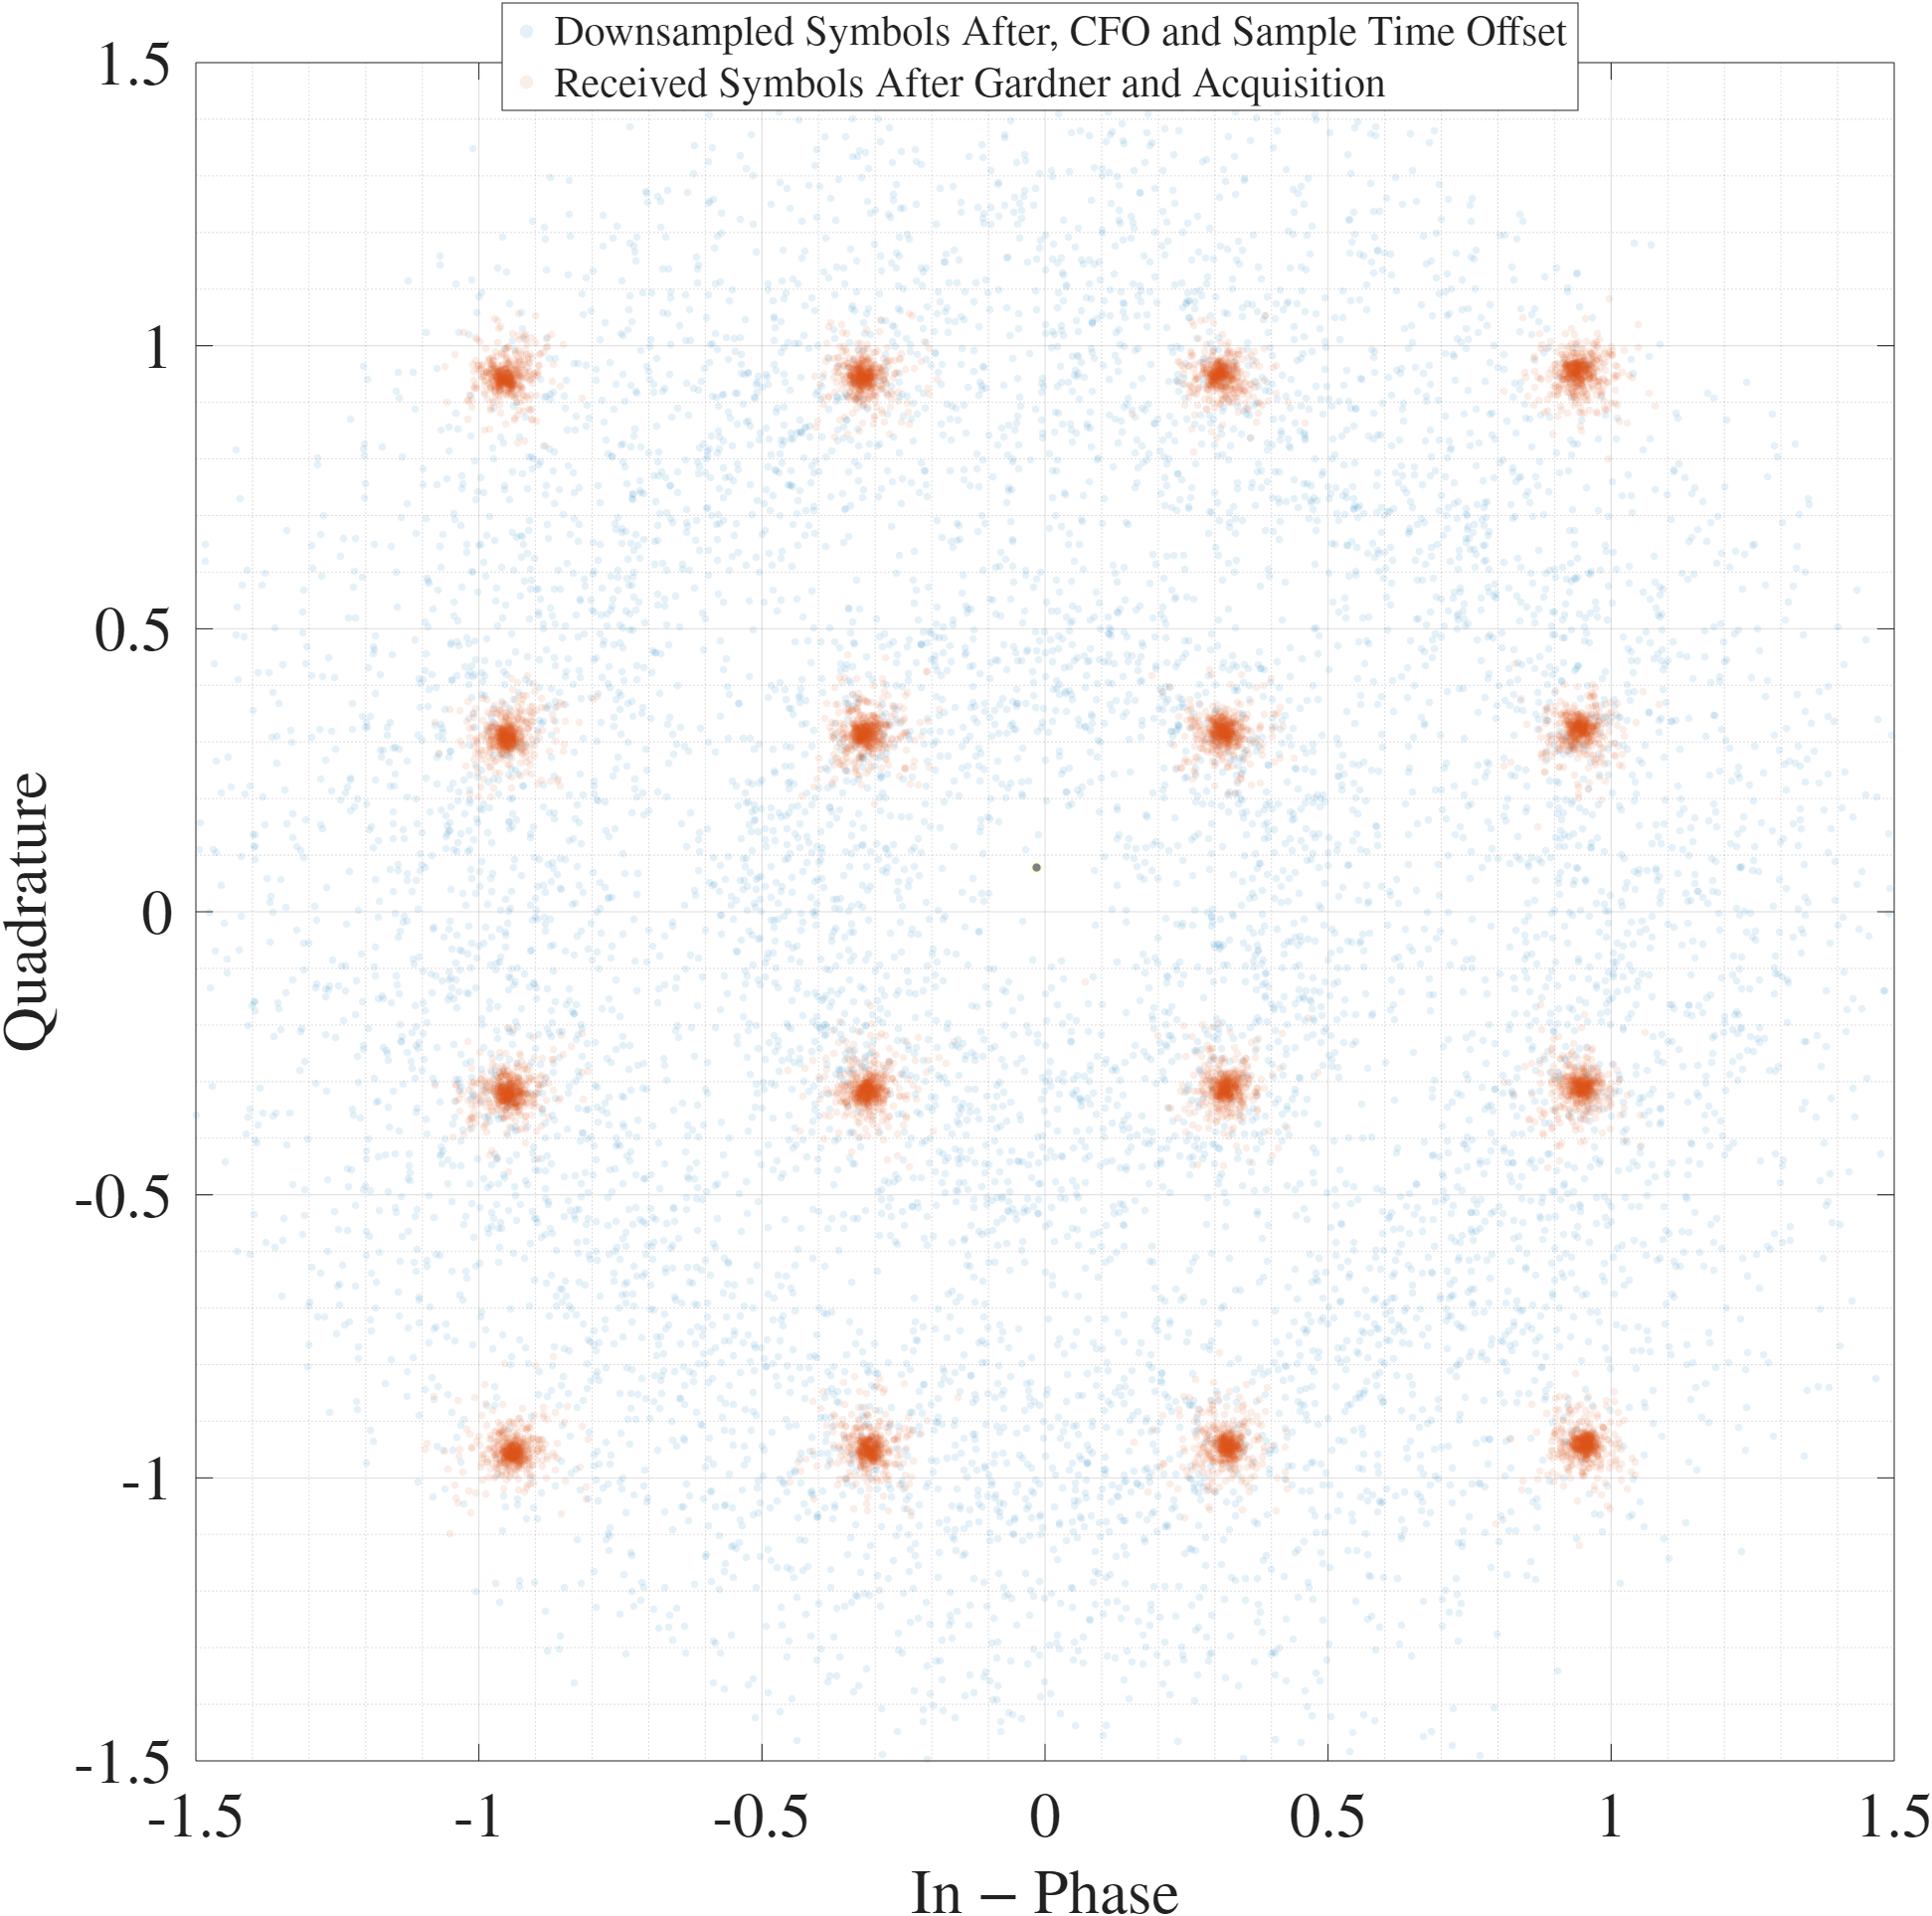
\includegraphics[width=0.7\linewidth]{Images/const-corrected.png} 
		\caption{Simulated 16-QAM constellation showing downsampled symbols affected by CFO and sample time offset  versus symbols after Gardner timing recovery and Frame/CFO acquisition with No Noise}
		\label{fig:const-corrected}
	\end{figure}
	
\end{document}